\documentclass[12pt,twoside,letterpaper]{article}
%NOTE: This report format is

\newcommand{\reporttitle}{{\huge \textsc{Rapport} \\ \vspace{0.5cm} {\Large Travail Pratique 1 : TravelHub}}}

\newcommand{\reportauthorOne}{Nom \& Prénom}
\newcommand{\reportauthorTwo}{Nom \& Prénom}
\newcommand{\reportauthorThree}{Nom \& Prénom}
% \newcommand{\cidOne}{your id number}
\newcommand{\reportProfessor}{Yacine Yaddaden, Ph. D.}
% \newcommand{\cidTwo}{your id number}
\newcommand{\reporttype}{Coursework}
\bibliographystyle{plain}

% Codage T1 : césure du français, guillemets et soulignés dans le code.
\usepackage[T1]{fontenc}

% include files that load packages and define macros
%%%%%%%%%%%%%%%%%%%%%%%%%%%%%%%%%%%%%%%%%
% University Assignment Title Page 
% LaTeX Template
% Version 1.0 (27/12/12)
%
% This template has been downloaded from:
% http://www.LaTeXTemplates.com
%
% Original author:
% WikiBooks (http://en.wikibooks.org/wiki/LaTeX/Title_Creation)
%
% License:
% CC BY-NC-SA 3.0 (http://creativecommons.org/licenses/by-nc-sa/3.0/)
% 
% Instructions for using this template:
% This title page is capable of being compiled as is. This is not useful for 
% including it in another document. To do this, you have two options: 
%
% 1) Copy/paste everything between \begin{document} and \end{document} 
% starting at \begin{titlepage} and paste this into another LaTeX file where you 
% want your title page.
% OR
% 2) Remove everything outside the \begin{titlepage} and \end{titlepage} and 
% move this file to the same directory as the LaTeX file you wish to add it to. 
% Then add \input{./title_page_1.tex} to your LaTeX file where you want your
% title page.
%
%----------------------------------------------------------------------------------------
%	PACKAGES AND OTHER DOCUMENT CONFIGURATIONS
%----------------------------------------------------------------------------------------
\usepackage{ifxetex}
\usepackage{textpos}
\usepackage{natbib}
\usepackage{kpfonts}
\usepackage[letterpaper,hmargin=2.8cm,vmargin=2.0cm,includeheadfoot]{geometry}
\usepackage{ifxetex}
\usepackage{stackengine}
\usepackage{tabularx,longtable,multirow,subfigure,caption}%hangcaption
\usepackage{fncylab} %formatting of labels
\usepackage{fancyhdr}
\usepackage{color}
\usepackage[tight,ugly]{units}
\usepackage{url}
\usepackage{float}
\usepackage[french]{babel}
\usepackage{amsmath}
\usepackage{graphicx}
\usepackage[colorinlistoftodos]{todonotes}
\usepackage{dsfont}
\usepackage{epstopdf} % automatically replace .eps with .pdf in graphics
\usepackage{natbib}
\usepackage{backref}
\usepackage{array}
\usepackage{latexsym}
\usepackage{etoolbox}

\usepackage{enumerate} % for numbering with [a)] format 



\ifxetex
\usepackage{fontspec}
\setmainfont[Scale=.8]{OpenDyslexic-Regular}
\else
\usepackage[pdftex,pagebackref,hypertexnames=false,colorlinks]{hyperref} % provide links in pdf
\hypersetup{pdftitle={},
  pdfsubject={}, 
  pdfauthor={\reportauthorOne},
  pdfkeywords={}, 
  pdfstartview=FitH,
  pdfpagemode={UseOutlines},% None, FullScreen, UseOutlines
  bookmarksnumbered=true, bookmarksopen=true, colorlinks,
    citecolor=black,%
    filecolor=black,%
    linkcolor=black,%
    urlcolor=black}
\usepackage[all]{hypcap}
\fi

\usepackage{tcolorbox}

% various theorems
\usepackage{ntheorem}
\theoremstyle{break}
\newtheorem{lemma}{Lemma}
\newtheorem{theorem}{Theorem}
\newtheorem{remark}{Remark}
\newtheorem{definition}{Definition}
\newtheorem{proof}{Proof}

% example-environment
\newenvironment{example}[1][]
{ 
\vspace{4mm}
\noindent\makebox[\linewidth]{\rule{\hsize}{1.5pt}}
\textbf{Example #1}\\
}
{ 
\noindent\newline\makebox[\linewidth]{\rule{\hsize}{1.0pt}}
}



%\renewcommand{\rmdefault}{pplx} % Palatino
% \renewcommand{\rmdefault}{put} % Utopia

\ifxetex
\else
\renewcommand*{\rmdefault}{bch} % Charter
\renewcommand*{\ttdefault}{cmtt} % Computer Modern Typewriter
%\renewcommand*{\rmdefault}{phv} % Helvetica
%\renewcommand*{\rmdefault}{iwona} % Avant Garde
\fi

\setlength{\parindent}{0em}  % indentation of paragraph

\setlength{\headheight}{14.5pt}
\pagestyle{fancy}
\fancyfoot[ER,OL]{\thepage}%Page no. in the left on
                                %odd pages and on right on even pages
\fancyfoot[OC,EC]{\sffamily }
\renewcommand{\headrulewidth}{0.1pt}
\renewcommand{\footrulewidth}{0.1pt}
\captionsetup{margin=10pt,font=small,labelfont=bf}


%--- chapter heading

\def\@makechapterhead#1{%
  \vspace*{10\p@}%
  {\parindent \z@ \raggedright %\sffamily
        %{\Large \MakeUppercase{\@chapapp} \space \thechapter}
        %\\
        %\hrulefill
        %\par\nobreak
        %\vskip 10\p@
    \interlinepenalty\@M
    \Huge \bfseries 
    \thechapter \space\space #1\par\nobreak
    \vskip 30\p@
  }}

%---chapter heading for \chapter*  
\def\@makeschapterhead#1{%
  \vspace*{10\p@}%
  {\parindent \z@ \raggedright
    \sffamily
    \interlinepenalty\@M
    \Huge \bfseries  
    #1\par\nobreak
    \vskip 30\p@
  }}
  



% %%%%%%%%%%%%% boxit
\def\Beginboxit
   {\par
    \vbox\bgroup
	   \hrule
	   \hbox\bgroup
		  \vrule \kern1.2pt %
		  \vbox\bgroup\kern1.2pt
   }

\def\Endboxit{%
			      \kern1.2pt
		       \egroup
		  \kern1.2pt\vrule
		\egroup
	   \hrule
	 \egroup
   }	

\newenvironment{boxit}{\Beginboxit}{\Endboxit}
\newenvironment{boxit*}{\Beginboxit\hbox to\hsize{}}{\Endboxit}



\allowdisplaybreaks

\makeatletter
\newcounter{elimination@steps}
\newcolumntype{R}[1]{>{\raggedleft\arraybackslash$}p{#1}<{$}}
\def\elimination@num@rights{}
\def\elimination@num@variables{}
\def\elimination@col@width{}
\newenvironment{elimination}[4][0]
{
    \setcounter{elimination@steps}{0}
    \def\elimination@num@rights{#1}
    \def\elimination@num@variables{#2}
    \def\elimination@col@width{#3}
    \renewcommand{\arraystretch}{#4}
    \start@align\@ne\st@rredtrue\m@ne
}
{
    \endalign
    \ignorespacesafterend
}
\newcommand{\eliminationstep}[2]
{
    \ifnum\value{elimination@steps}>0\leadsto\quad\fi
    \left[
        \ifnum\elimination@num@rights>0
            \begin{array}
            {@{}*{\elimination@num@variables}{R{\elimination@col@width}}
            |@{}*{\elimination@num@rights}{R{\elimination@col@width}}}
        \else
            \begin{array}
            {@{}*{\elimination@num@variables}{R{\elimination@col@width}}}
        \fi
            #1
        \end{array}
    \right]
    & 
    \begin{array}{l}
        #2
    \end{array}
    &%                                    moved second & here
    \addtocounter{elimination@steps}{1}
}
\makeatother

%% Fast macro for column vectors
\makeatletter  
\def\colvec#1{\expandafter\colvec@i#1,,,,,,,,,\@nil}
\def\colvec@i#1,#2,#3,#4,#5,#6,#7,#8,#9\@nil{% 
  \ifx$#2$ \begin{bmatrix}#1\end{bmatrix} \else
    \ifx$#3$ \begin{bmatrix}#1\\#2\end{bmatrix} \else
      \ifx$#4$ \begin{bmatrix}#1\\#2\\#3\end{bmatrix}\else
        \ifx$#5$ \begin{bmatrix}#1\\#2\\#3\\#4\end{bmatrix}\else
          \ifx$#6$ \begin{bmatrix}#1\\#2\\#3\\#4\\#5\end{bmatrix}\else
            \ifx$#7$ \begin{bmatrix}#1\\#2\\#3\\#4\\#5\\#6\end{bmatrix}\else
              \ifx$#8$ \begin{bmatrix}#1\\#2\\#3\\#4\\#5\\#6\\#7\end{bmatrix}\else
                 \PackageError{Column Vector}{The vector you tried to write is too big, use bmatrix instead}{Try using the bmatrix environment}
              \fi
            \fi
          \fi
        \fi
      \fi
    \fi
  \fi 
}  
\makeatother

\robustify{\colvec}

%%% Local Variables: 
%%% mode: latex
%%% TeX-master: "notes"
%%% End: 
 % various packages needed for maths etc.

% Paquets et macros du contenu (listings, TikZ, tableaux, captures) ;
% la mise en page du modèle n'est pas modifiée.
%----------------------------------------------------------------------------------------
%	Paquets et macros du contenu du rapport TravelHub.
%	Chargé après includes.tex : la mise en page du modèle reste inchangée.
%----------------------------------------------------------------------------------------
\usepackage{listings}
\usepackage{booktabs}
% Colonnes X alignées à gauche : pas d'espaces étirés dans les cellules étroites.
\renewcommand{\tabularxcolumn}[1]{>{\raggedright\arraybackslash}p{#1}}
\usepackage{tikz}
% babel : neutralise les caractères actifs du français (: ; ! ?) dans les figures TikZ.
\usetikzlibrary{positioning,arrows.meta,shapes.multipart,babel}

% Code en ligne : identifiants, chemins, noms de contraintes (_ { } sans échappement).
% Coupure de ligne permise après « _ », « . » et « / » : les longs identifiants
% (trips_participant_single_owner, apps.core.exceptions…) ne débordent pas.
\ExplSyntaxOn
\tl_new:N \l__th_code_tl
\NewDocumentCommand{\code}{m}{
  \tl_set:Ne \l__th_code_tl { \tl_to_str:n {#1} }
  \regex_replace_all:nnN { ([\_\./]) } { \1 \c{allowbreak} } \l__th_code_tl
  \regex_replace_once:nnN { \c{allowbreak} \Z } { } \l__th_code_tl
  \texttt{ \l__th_code_tl }
}
\ExplSyntaxOff
% Les mots en chasse fixe sont larges : souplesse supplémentaire pour les seuls
% paragraphes qui déborderaient sinon.
\setlength{\emergencystretch}{3em}

% Capture d'écran : l'image figures/<fichier> si elle existe, sinon un cadre qui
% indique le fichier attendu (le document compile avant l'ajout des captures).
\newcommand{\capture}[3]{%
  \begin{figure}[H]
    \centering
    \IfFileExists{figures/#1}{%
      \includegraphics[width=\linewidth,height=0.42\textheight,keepaspectratio]{figures/#1}%
    }{%
      \fbox{\parbox[c][4cm][c]{0.9\linewidth}{\centering\small
        Capture à insérer :\\[2pt] \texttt{figures/#1}}}%
    }
    \caption{#2}\label{#3}
  \end{figure}}

% Extraits de code
\definecolor{codegris}{gray}{0.45}
\definecolor{codebleu}{rgb}{0.10,0.25,0.55}
\definecolor{codevert}{rgb}{0.10,0.45,0.20}
\definecolor{codefond}{gray}{0.97}

\renewcommand{\lstlistingname}{Extrait}
% Un extrait n'est jamais coupé entre deux pages (ils font tous moins d'une page).
\BeforeBeginEnvironment{lstlisting}{\par\noindent\begin{minipage}{\linewidth}}
\AfterEndEnvironment{lstlisting}{\end{minipage}\par\smallskip}
\renewcommand{\lstlistlistingname}{Liste des extraits}

\lstdefinelanguage{json}{
  morestring=[b]",
  sensitive=true,
}
\lstdefinelanguage{graphql}{
  morekeywords={query,mutation,fragment,on,true,false,null},
  sensitive=true,
  morecomment=[l]{\#},
  morestring=[b]",
}

\lstset{
  basicstyle=\ttfamily\scriptsize,
  keywordstyle=\color{codebleu},
  commentstyle=\color{codegris}\itshape,
  stringstyle=\color{codevert},
  backgroundcolor=\color{codefond},
  frame=single,
  rulecolor=\color{black!25},
  framesep=3pt,
  xleftmargin=4pt,
  xrightmargin=4pt,
  columns=fullflexible,
  keepspaces=true,
  showstringspaces=false,
  breaklines=true,
  breakatwhitespace=true,
  tabsize=4,
  captionpos=t,
  aboveskip=8pt,
  belowskip=6pt,
  upquote=false,
  extendedchars=true,
  literate=
    {é}{{\'e}}1 {è}{{\`e}}1 {ê}{{\^e}}1 {ë}{{\"e}}1
    {à}{{\`a}}1 {â}{{\^a}}1 {ç}{{\c{c}}}1 {î}{{\^i}}1 {ï}{{\"i}}1
    {ô}{{\^o}}1 {ù}{{\`u}}1 {û}{{\^u}}1
    {É}{{\'E}}1 {À}{{\`A}}1 {Ç}{{\c{C}}}1
    {«}{{\guillemotleft}}1 {»}{{\guillemotright}}1
    {’}{{'}}1 {—}{{---}}1 {…}{{...}}1 {→}{{$\rightarrow$}}1,
}

% Diagrammes
\tikzset{
  entite/.style={
    draw, thick, rectangle split, rectangle split parts=2,
    rectangle split part fill={black!10,white},
    rectangle split part align={center,left},
    text width=4.3cm, inner sep=3pt, font=\scriptsize\ttfamily},
  rel/.style={thick, -{Latex[length=2mm]}},
  card/.style={font=\scriptsize, inner sep=1.5pt},
  etape/.style={draw, rounded corners=2pt, fill=black!4, text width=6.2cm,
    align=center, font=\small, minimum height=0.75cm},
  note/.style={font=\scriptsize, text width=6.4cm, align=left},
}



%%%%%%%%%%%%%%%%%%%%%%%%%%%%

\begin{document}
% front page
% Last modification: 2016-09-29 (Marc Deisenroth)
% Modification for UW: 2017-05-22 (jphickey)
\begin{titlepage}

\newcommand{\HRule}{\rule{\linewidth}{0.5mm}} % Defines a new command for the horizontal lines, change thickness here


%----------------------------------------------------------------------------------------
%	LOGO SECTION
%----------------------------------------------------------------------------------------



\begin{center} % Center remainder of the page

%----------------------------------------------------------------------------------------
%	HEADING SECTIONS
%----------------------------------------------------------------------------------------


\includegraphics[width=7cm]{uqar}\\[1.5cm] 
\textbf{\textsc{\Large Technologies de l'inforoute \\ \vspace{0.5cm} INF37407 (MS)}}\\[1.0cm] 
\textsc{\Large Université du Québec à Rimouski - Campus Lévis}\\[0.5cm] 
\textsc{\large Département de mathématiques, d'informatique et de génie}\\[0.95cm] 

%----------------------------------------------------------------------------------------
%	TITLE SECTION
%----------------------------------------------------------------------------------------

\HRule \\ % [0.4cm]
{ \huge \bfseries \reporttitle}\\ % Title of your document
\HRule \\[1.5cm]
\end{center}
%----------------------------------------------------------------------------------------
%	AUTHOR SECTION
%----------------------------------------------------------------------------------------

%\begin{minipage}{0.4\hsize}
\begin{flushleft} \large
\textit{\textsc{\textbf{Équipe :}}}\\
\reportauthorOne \\ %~(Matricule: \cidOne)\\ % 
\reportauthorTwo \\
\reportauthorThree \\
\vspace{0.5cm}
\textit{\textsc{\textbf{Professeur :}}}\\
\reportProfessor
\end{flushleft}
% \vspace{3.5cm}
\vfill
\makeatletter
Date: \@date 

% \vfill % Fill the rest of the page with whitespace



\makeatother


\end{titlepage}




%%%%%%%%%%%%%%%%%%%%%%%%%%% table of content
%If a table of content is needed, simply uncomment the following lines
\tableofcontents
\newpage

%%%%%%%%%%%%%%%%%%%%%%%%%%%% Main document
%========================================================================================
\section{Introduction}
\label{sec:introduction}
%========================================================================================

\subsection{Contexte}

TravelHub est une plateforme qui sert à planifier des voyages à plusieurs. Un utilisateur crée un voyage et le découpe en destinations. Il prévoit ensuite des activités à chaque étape. Il peut aussi partager son voyage avec d'autres utilisateurs en leur donnant un rôle, qui peut être propriétaire, éditeur ou lecteur. Pour chaque destination, l'application va chercher la météo du séjour et quelques informations sur le pays.

Dans ce rapport, nous présentons le back-end que nous avons réalisé pour le premier travail pratique. Nous expliquons nos choix techniques, l'architecture, le modèle de données et les deux API. Nous parlons aussi de l'intégration des services externes, de la sécurité et des tests. Tout ce qui est décrit ici se retrouve dans le code du dépôt.

\subsection{Objectifs}

Nous nous sommes fixé six objectifs :
\begin{itemize}
  \item modéliser les données dans PostgreSQL avec des relations 1-N et N-N, et laisser la base vérifier elle-même les contraintes d'intégrité ;
  \item offrir les mêmes fonctions avec une API REST (Django REST Framework) et avec une API GraphQL (Graphene-Django) ;
  \item utiliser deux API publiques, Open-Meteo (REST) et Countries (GraphQL) ;
  \item protéger l'accès avec des jetons JWT et des permissions basées sur le rôle, en suivant l'OWASP API Security Top 10~\cite{owasp} ;
  \item garder des données cohérentes grâce à plusieurs niveaux de validation et aux transactions ;
  \item tout vérifier avec des tests automatisés et une collection Postman.
\end{itemize}

\subsection{Périmètre}

Le TP1 porte seulement sur le back-end, l'interface utilisateur viendra au TP2. Pour l'instant, l'API est donc la seule façon d'utiliser le système. On peut la tester avec Swagger UI, GraphiQL, Postman et l'administration de Django. Nous avons aussi ajouté une image Docker, de l'intégration continue, des journaux structurés et des sauvegardes. L'énoncé ne le demandait pas, mais cela nous servira pour déployer le TP2.

\subsection{Organisation du rapport}

La section~\ref{sec:environnement} explique les versions que nous avons choisies. Les sections~\ref{sec:architecture} et~\ref{sec:modele} présentent l'architecture et le modèle de données, puis la section~\ref{sec:gestion} décrit la logique métier. La section~\ref{sec:integrations} parle des services externes. Les deux API sont présentées et comparées aux sections~\ref{sec:rest} et~\ref{sec:graphql}. Les sections~\ref{sec:validation} à~\ref{sec:tests} traitent de l'intégrité, de la sécurité et des tests. Enfin, la section~\ref{sec:industrialisation} porte sur le déploiement et la section~\ref{sec:conclusion} conclut le rapport.

%========================================================================================
\section{Environnement et technologies}
\label{sec:environnement}
%========================================================================================

\subsection{Versions retenues}

Le tableau~\ref{tab:versions} donne les versions fixées dans \code{requirements.txt} et \code{requirements-dev.txt}. Chaque dépendance a une version exacte. Deux installations donnent donc le même environnement.

\begin{table}[H]
  \centering
  \small
  \caption{Versions des outils et des bibliothèques.}
  \label{tab:versions}
  \begin{tabularx}{\linewidth}{@{}l l X@{}}
    \toprule
    \textbf{Composant} & \textbf{Version} & \textbf{Rôle} \\
    \midrule
    Python & 3.14 & Langage \\
    PostgreSQL & 18 & Base de données relationnelle~\cite{postgresql} \\
    Django & 5.2.18 (LTS) & Cadriciel web, ORM, administration~\cite{django} \\
    Django REST Framework & 3.18.3 & API REST~\cite{drf} \\
    SimpleJWT & 5.5.1 & Jetons JWT et liste noire des jetons révoqués~\cite{simplejwt} \\
    drf-spectacular & 0.30.0 & Schéma OpenAPI 3, Swagger UI, ReDoc~\cite{spectacular} \\
    Graphene-Django & 3.2.3 & API GraphQL~\cite{graphene} \\
    django-filter & 26.2 & Filtres des listes \\
    django-cors-headers & 4.9.0 & Politique CORS \\
    django-environ & 0.14.0 & Configuration par variables d'environnement \\
    psycopg & 3.3.6 & Pilote PostgreSQL \\
    requests & 2.34.2 & Appels HTTP vers les services externes \\
    Gunicorn, WhiteNoise & 26.2.0, 6.12.0 & Serveur WSGI et fichiers statiques en production \\
    \midrule
    pytest, pytest-django & 9.1.1, 4.14.0 & Tests \\
    pytest-cov & 7.1.0 & Couverture de code \\
    responses & 0.26.3 & Simulation des appels HTTP externes \\
    Ruff & 0.17.1 & Analyse statique et formatage \\
    \bottomrule
  \end{tabularx}
\end{table}

Nous avons développé sous Windows 11. Les scripts d'exploitation sont donc en PowerShell, et nous avons géré la base avec pgAdmin~4.

\subsection{Pourquoi Django 5.2 LTS}

Nous voulions la dernière version stable de Django qui marche avec \emph{toutes} nos dépendances. Django 6.1 était déjà sorti, mais Graphene-Django 3.2.3 et SimpleJWT 5.5.1 ne disent pas encore supporter Django~6. Django 5.2 est une version LTS, maintenue jusqu'en avril 2028, et elle supporte officiellement Python 3.14. Nous avons préféré un ensemble stable à la version la plus récente du cadriciel.

\subsection{Configuration}

Les paramètres sont répartis dans quatre modules (tableau~\ref{tab:settings}). Les valeurs sensibles ne sont jamais écrites dans le code. \code{django-environ} les lit dans l'environnement, sinon dans un fichier \code{.env} que Git ignore. Toutes les variables sont expliquées dans \code{.env.example}.

\begin{table}[H]
  \centering
  \small
  \caption{Modules de paramètres.}
  \label{tab:settings}
  \begin{tabularx}{\linewidth}{@{}l X@{}}
    \toprule
    \textbf{Module} & \textbf{Usage} \\
    \midrule
    \code{config.settings.base} & Paramètres communs (applications, DRF, JWT, GraphQL, journaux) \\
    \code{config.settings.dev} & Développement, avec \code{DEBUG}, GraphiQL et l'introspection activés \\
    \code{config.settings.test} & Tests, avec un hachage rapide des mots de passe, un cache en mémoire et les journaux sur la console \\
    \code{config.settings.prod} & Production, avec HTTPS, HSTS, cookies sécurisés, JSON seulement et WhiteNoise \\
    \bottomrule
  \end{tabularx}
\end{table}

%========================================================================================
\section{Architecture}
\label{sec:architecture}
%========================================================================================

\subsection{Applications Django}

Le projet suit la structure recommandée par Django : un projet de configuration (\code{config}) et des applications à responsabilité unique, regroupées sous \code{apps/} (tableau~\ref{tab:apps}).

\begin{table}[H]
  \centering
  \small
  \caption{Applications du projet.}
  \label{tab:apps}
  \begin{tabularx}{\linewidth}{@{}l X@{}}
    \toprule
    \textbf{Application} & \textbf{Responsabilité} \\
    \midrule
    \code{config} & Paramètres, routage principal, schéma GraphQL racine, points d'entrée WSGI et ASGI \\
    \code{apps.core} & Éléments transversaux : \code{TimeStampedModel}, permissions par rôle, gestionnaire d'exceptions, vue GraphQL, journaux, contrôle de santé \\
    \code{apps.accounts} & Utilisateur personnalisé, inscription, jetons JWT, profil \\
    \code{apps.trips} & Voyages et participants, services métier (création, clonage, statistiques) \\
    \code{apps.itinerary} & Destinations et activités, coordonnées géographiques \\
    \code{apps.integrations} & Clients Open-Meteo et Countries, couche HTTP commune, agrégateur \\
    \bottomrule
  \end{tabularx}
\end{table}

Chaque application métier contient les mêmes fichiers : \code{models.py}, \code{serializers.py}, \code{views.py}, \code{urls.py}, \code{filters.py}, \code{schema.py} (GraphQL), \code{admin.py}, \code{services.py} et un dossier \code{tests/}. Cette régularité facilite la navigation dans le code.

\subsection{Arborescence}

\begin{lstlisting}[language={},caption={Arborescence du dépôt (simplifiée).},label={lst:arbo}]
TravelHub/
|-- config/              settings/ (base, dev, test, prod), urls.py, schema.py
|-- apps/
|   |-- core/            permissions, exceptions, vue GraphQL, journaux
|   |-- accounts/        User, inscription, JWT
|   |-- trips/           Trip, TripParticipant, services
|   |-- itinerary/       Destination, Activity
|   `-- integrations/    services/ (http, open_meteo, countries, aggregator)
|-- postman/             collection v2.1 et environnement
|-- scripts/             backup.ps1, restore.ps1, db/
|-- .github/workflows/   ci.yml
|-- Dockerfile  docker-compose.yml  gunicorn.conf.py
`-- requirements.txt  requirements-dev.txt  pytest.ini  .env.example
\end{lstlisting}

\subsection{Répartition des responsabilités}

Le code respecte quatre principes.
\begin{enumerate}
  \item \textbf{Des vues minces.} Une vue authentifie, choisit le queryset, applique la permission, puis délègue. Elle ne contient pas de règle métier.
  \item \textbf{Des services explicites.} Les opérations qui touchent plusieurs tables (\code{create_trip}, \code{clone_trip}, \code{add_participant}) vivent dans \code{services.py}. Les API REST et GraphQL les appellent toutes deux.
  \item \textbf{Des règles portées par le modèle et par la base.} Les règles de dates sont écrites dans \code{Model.clean()}. Les invariants sont doublés par des contraintes PostgreSQL.
  \item \textbf{Des erreurs centralisées.} Un gestionnaire unique (\code{apps/core/exceptions.py}) produit la même enveloppe JSON pour toutes les erreurs.
\end{enumerate}

\subsection{Flux d'une requête}

La figure~\ref{fig:flux} suit une requête \code{PATCH /api/trips/12/} de bout en bout.

\begin{figure}[tbp]
  \centering
  \begin{tikzpicture}[node distance=0.32cm]
    \node[etape] (client) {Client HTTP (\texttt{Authorization: Bearer} \ldots)};
    \node[etape, below=of client] (mw) {Intergiciels : \texttt{RequestIdMiddleware}, sécurité, CORS};
    \node[etape, below=of mw] (url) {Routage : \texttt{config/urls.py} $\rightarrow$ routeur DRF};
    \node[etape, below=of url] (auth) {\texttt{TripViewSet} : authentification JWT, limites de requêtes, \texttt{IsAuthenticated}};
    \node[etape, below=of auth] (qs) {\texttt{get\_queryset()} : \texttt{Trip.objects.visible\_to(user)}};
    \node[etape, below=of qs] (perm) {Permission objet : \texttt{IsTripEditor}};
    \node[etape, below=of perm] (ser) {Serializer : \texttt{validate()}, puis \texttt{Model.clean()} et contraintes};
    \node[etape, below=of ser] (db) {ORM $\rightarrow$ PostgreSQL (contraintes \texttt{CHECK}, \texttt{UNIQUE})};
    \node[etape, below=of db] (rep) {Réponse JSON, en-tête \texttt{X-Request-ID}, ligne de journal};

    \foreach \a/\b in {client/mw, mw/url, url/auth, auth/qs, qs/perm, perm/ser, ser/db, db/rep}
      \draw[rel] (\a) -- (\b);

    \node[note, right=0.5cm of auth] {Jeton absent ou invalide : \textbf{401}. Quota dépassé : \textbf{429}.};
    \node[note, right=0.5cm of qs] {Voyage d'un autre utilisateur : absent du queryset, donc \textbf{404}.};
    \node[note, right=0.5cm of perm] {Lecteur qui tente une modification : \textbf{403}.};
    \node[note, right=0.5cm of ser] {Dates incohérentes : \textbf{400} avec le détail par champ.};
    \node[note, right=0.5cm of db] {Contrainte violée (accès concurrent) : \code{IntegrityError} convertie en \textbf{400}.};
  \end{tikzpicture}
  \caption{Traitement d'une modification de voyage. Toute exception est convertie par \texttt{exception\_handler} en enveloppe \texttt{\{"error": \ldots\}}.}
  \label{fig:flux}
\end{figure}

L'ordre de ces étapes porte la sécurité. Le filtrage par \code{visible_to()} précède la permission objet. Un voyage d'autrui n'existe donc pas pour l'utilisateur : il reçoit 404, et non 403, ce qui ne révèle pas l'existence de la ressource.

%========================================================================================
\section{Modèle de données}
\label{sec:modele}
%========================================================================================

\subsection{Diagramme entité-association}

Le modèle compte cinq tables métier (figure~\ref{fig:erd}). Les tables techniques de Django et de SimpleJWT (sessions, permissions, liste noire des jetons) n'y figurent pas. Les champs \code{created_at} et \code{updated_at} proviennent du modèle abstrait \code{TimeStampedModel} de \code{apps.core}.

\begin{figure}[tbp]
  \centering
  \resizebox{\linewidth}{!}{%
  \begin{tikzpicture}
    \node[entite] (trip) at (0,0) {%
      \textbf{trips\_trip}
      \nodepart{two}
      id \hfill bigint PK\\
      owner\_id \hfill FK user\\
      title \hfill varchar(200)\\
      description \hfill text\\
      start\_date \hfill date\\
      end\_date \hfill date\\
      status \hfill varchar(20)\\
      budget \hfill numeric(10,2) NULL\\
      created\_at, updated\_at};

    \node[entite, right=1.3cm of trip.north east, anchor=north west] (dest) {%
      \textbf{itinerary\_destination}
      \nodepart{two}
      id \hfill bigint PK\\
      trip\_id \hfill FK trip\\
      city, country \hfill varchar(120)\\
      country\_code \hfill varchar(2)\\
      arrival\_date \hfill date\\
      departure\_date \hfill date\\
      order \hfill smallint\\
      latitude \hfill numeric(9,6) NULL\\
      longitude \hfill numeric(9,6) NULL\\
      created\_at, updated\_at};

    \node[entite, below=1.9cm of trip] (part) {%
      \textbf{trips\_tripparticipant}
      \nodepart{two}
      id \hfill bigint PK\\
      trip\_id \hfill FK trip\\
      user\_id \hfill FK user\\
      role \hfill varchar(10)\\
      joined\_at \hfill timestamptz\\
      invited\_by\_id \hfill FK user NULL};

    \node[entite, below=1.9cm of dest] (act) {%
      \textbf{itinerary\_activity}
      \nodepart{two}
      id \hfill bigint PK\\
      destination\_id \hfill FK destination\\
      name \hfill varchar(200)\\
      description \hfill text\\
      category \hfill varchar(20)\\
      date \hfill date\\
      start\_time \hfill time NULL\\
      cost \hfill numeric(10,2)\\
      created\_at, updated\_at};

    \node[entite, left=1.3cm of trip.south west, anchor=east, yshift=-1.2cm] (user) {%
      \textbf{accounts\_user}
      \nodepart{two}
      id \hfill bigint PK\\
      username \hfill varchar(150) UQ\\
      email \hfill UQ sur lower(email)\\
      password \hfill varchar(128)\\
      first\_name, last\_name\\
      is\_active, is\_staff,\\
      is\_superuser\\
      date\_joined, last\_login};

    % User 1 -- N Trip (propriétaire)
    \draw[rel] (user.north) |- node[card, pos=0.94, above] {0..*} node[card, pos=0.06, left] {1}
      node[card, pos=0.75, above] {owner} (trip.west);
    % User 1 -- N TripParticipant (participant)
    \draw[rel] (user.east) -- node[card, pos=0.5, above] {1} ++(0.6,0)
      |- node[card, pos=0.25, right] {user} node[card, pos=0.93, above] {0..*}
      ([yshift=0.3cm]part.west);
    % User 0..1 -- N TripParticipant (invité par)
    \draw[rel, dashed] (user.south) |- node[card, pos=0.06, left] {0..1}
      node[card, pos=0.7, below] {invited\_by} node[card, pos=0.95, below] {0..*}
      ([yshift=-0.4cm]part.west);
    % Trip 1 -- N TripParticipant
    \draw[rel] (trip.south) -- node[card, pos=0.12, right] {1} node[card, pos=0.88, right] {0..*}
      node[card, pos=0.5, left] {trip} (part.north);
    % Trip 1 -- N Destination
    \draw[rel] (trip.east) -- node[card, pos=0.15, above] {1} node[card, pos=0.75, above] {0..*}
      node[card, pos=0.45, below] {trip} (trip.east -| dest.west);
    % Destination 1 -- N Activity
    \draw[rel] (dest.south) -- node[card, pos=0.12, right] {1} node[card, pos=0.88, right] {0..*}
      node[card, pos=0.5, left] {destination} (act.north);
  \end{tikzpicture}}
  \caption{Modèle de données de TravelHub. Les flèches vont de la table référencée vers la table qui porte la clé étrangère. La relation N-N entre utilisateurs et voyages passe par \texttt{trips\_tripparticipant}.}
  \label{fig:erd}
\end{figure}

La figure~\ref{fig:erd-pgadmin} montre le même schéma, produit par l'outil ERD de pgAdmin à partir de la base réelle.

\capture{erd-pgadmin.png}{Diagramme ERD généré par pgAdmin~4 (\emph{Tools} $\rightarrow$ \emph{ERD Tool}) sur la base \texttt{travelhub}.}{fig:erd-pgadmin}

\subsection{Relations}

Le tableau~\ref{tab:relations} détaille chaque relation. Le nom inverse (\code{related_name}) est choisi pour se lire naturellement : \code{user.owned_trips}, \code{trip.destinations}, \code{destination.activities}.

\begin{table}[H]
  \centering
  \small
  \caption{Relations du modèle.}
  \label{tab:relations}
  \begin{tabularx}{\linewidth}{@{}l l l X@{}}
    \toprule
    \textbf{Relation} & \textbf{Type} & \textbf{Suppression} & \textbf{Accès inverse} \\
    \midrule
    \code{Trip.owner} $\rightarrow$ \code{User} & 1-N & \code{CASCADE} & \code{user.owned_trips} \\
    \code{Trip.participants} $\leftrightarrow$ \code{User} & N-N & --- & \code{user.trips}, via \code{TripParticipant} \\
    \code{TripParticipant.trip} $\rightarrow$ \code{Trip} & 1-N & \code{CASCADE} & \code{trip.memberships} \\
    \code{TripParticipant.user} $\rightarrow$ \code{User} & 1-N & \code{CASCADE} & \code{user.trip_memberships} \\
    \code{TripParticipant.invited_by} $\rightarrow$ \code{User} & 1-N & \code{SET_NULL} & \code{user.sent_trip_invitations} \\
    \code{Destination.trip} $\rightarrow$ \code{Trip} & 1-N & \code{CASCADE} & \code{trip.destinations} \\
    \code{Activity.destination} $\rightarrow$ \code{Destination} & 1-N & \code{CASCADE} & \code{destination.activities} \\
    \bottomrule
  \end{tabularx}
\end{table}

La relation N-N mérite une précision. Une simple table de jointure ne suffit pas : l'association porte des attributs (rôle, date d'ajout, auteur de l'invitation). Elle est donc modélisée par un modèle intermédiaire explicite, déclaré avec \code{through}. Comme \code{TripParticipant} possède deux clés étrangères vers \code{User}, l'option \code{through_fields} désigne celles qui relient le voyage à ses participants.

\begin{lstlisting}[language=Python,caption={Relation N-N avec modèle intermédiaire (\texttt{apps/trips/models.py}, extrait).},label={lst:m2m}]
participants = models.ManyToManyField(
    settings.AUTH_USER_MODEL,
    through="TripParticipant",
    # TripParticipant a deux FK vers User (user, invited_by) : on indique lesquelles
    # relient le voyage à ses participants.
    through_fields=("trip", "user"),
    related_name="trips",
)
\end{lstlisting}

La suppression en cascade suit la composition : un voyage possède ses destinations, qui possèdent leurs activités. En revanche, la suppression de l'auteur d'une invitation ne doit pas retirer le participant invité ; \code{invited_by} passe alors à \code{NULL}.

\subsection{Utilisateur personnalisé}

Le modèle \code{accounts.User} hérite d'\code{AbstractUser}. Il a été déclaré dans \code{AUTH_USER_MODEL} avant la première migration, comme le recommande Django : changer de modèle utilisateur après coup est très coûteux. Le courriel est obligatoire et unique sans tenir compte de la casse, grâce à une contrainte d'unicité sur l'expression \code{Lower("email")}. Le courriel est aussi normalisé en minuscules dans \code{save()}, car \code{createsuperuser} n'appelle pas \code{clean()}.

\subsection{Contraintes d'intégrité}

Les règles essentielles sont vérifiées par PostgreSQL lui-même (tableau~\ref{tab:contraintes}). La base reste ainsi cohérente même si une écriture contourne la validation applicative, par exemple lors de deux requêtes simultanées. Chaque contrainte porte un nom et un message d'erreur en français, réutilisé par le gestionnaire d'exceptions (section~\ref{sec:validation}).

\begin{table}[H]
  \centering
  \small
  \caption{Contraintes déclarées dans les modèles.}
  \label{tab:contraintes}
  \begin{tabularx}{\linewidth}{@{}l l X@{}}
    \toprule
    \textbf{Nom} & \textbf{Type} & \textbf{Règle} \\
    \midrule
    \code{accounts_user_email_ci_unique} & \code{UNIQUE} & \code{lower(email)} unique \\
    \code{trips_trip_end_after_start} & \code{CHECK} & \code{end_date >= start_date} \\
    \code{trips_trip_budget_non_negative} & \code{CHECK} & budget nul ou positif \\
    \code{trips_trip_status_valid} & \code{CHECK} & statut parmi les cinq valeurs \\
    \code{trips_participant_unique_trip_user} & \code{UNIQUE} & un utilisateur au plus une fois par voyage \\
    \code{trips_participant_single_owner} & \code{UNIQUE} partiel & un seul \code{owner} par voyage (\code{WHERE role = 'owner'}) \\
    \code{trips_participant_role_valid} & \code{CHECK} & rôle parmi \code{owner}, \code{editor}, \code{viewer} \\
    \code{itinerary_destination_unique_trip_order} & \code{UNIQUE} & une position par destination dans un voyage \\
    \code{itinerary_destination_departure_after_arrival} & \code{CHECK} & \code{departure_date >= arrival_date} \\
    \code{itinerary_destination_country_code_iso2} & \code{CHECK} & code pays conforme à \code{^[A-Z]{2}$} \\
    \code{itinerary_destination_coordinates_valid} & \code{CHECK} & latitude et longitude fournies ensemble, dans leurs bornes \\
    \code{itinerary_activity_cost_non_negative} & \code{CHECK} & \code{cost >= 0} \\
    \code{itinerary_activity_category_valid} & \code{CHECK} & catégorie parmi les huit valeurs \\
    \bottomrule
  \end{tabularx}
\end{table}

Deux points de conception méritent d'être relevés. D'abord, la contrainte \code{trips_participant_single_owner} est un index unique \emph{partiel} : il ne porte que sur les lignes où \code{role = 'owner'}. Ensuite, la contrainte sur les coordonnées teste explicitement \code{IS NOT NULL}. En SQL, une condition \code{CHECK} évaluée à \code{NULL} est considérée comme respectée ; sans ce test, une latitude seule passerait.

\begin{lstlisting}[language=Python,caption={Contraintes du voyage (\texttt{apps/trips/models.py}, extrait).},label={lst:contraintes}]
class Meta:
    ordering = ["start_date", "pk"]
    indexes = [models.Index(fields=["start_date"], name="trips_trip_start_date_idx")]
    constraints = [
        models.CheckConstraint(
            condition=Q(end_date__gte=F("start_date")),
            name="trips_trip_end_after_start",
            violation_error_message=(
                "La date de fin doit être postérieure ou égale à la date de début."
            ),
        ),
        models.CheckConstraint(
            condition=Q(budget__isnull=True) | Q(budget__gte=0),
            name="trips_trip_budget_non_negative",
            violation_error_message="Le budget ne peut pas être négatif.",
        ),
        # ... trips_trip_status_valid
    ]
\end{lstlisting}

Les montants utilisent \code{DecimalField} (\code{numeric} en SQL) et jamais \code{float} : un coût de 0,10~\$ doit rester exact. Les choix (statut, rôle, catégorie) sont des \code{TextChoices} ; ils sont doublés d'une contrainte \code{CHECK}, car Django ne vérifie les choix qu'à la validation, jamais en base.

\subsection{Migrations}

Chaque application possède une migration initiale (\code{0001_initial.py}), générée par Django 5.2.18 avec \code{makemigrations}. La commande \code{sqlmigrate} permet de relire le SQL produit, notamment les contraintes et l'index partiel. La commande \code{migrate --check} sert à vérifier qu'une base restaurée est à jour (section~\ref{sec:industrialisation}). Dans Docker, le service \code{web} applique les migrations à chaque démarrage, avant de lancer Gunicorn.

%========================================================================================
\section{Gestion des voyages, destinations, activités et \mbox{participants}}
\sectionmark{Voyages et participants}
\label{sec:gestion}
%========================================================================================

\subsection{QuerySets réutilisables}

Les requêtes fréquentes sont regroupées dans un \code{QuerySet} personnalisé, exposé par \code{Trip.objects} (\code{TripQuerySet.as_manager()}). Elles se combinent par chaînage.

\begin{table}[H]
  \centering
  \small
  \caption{Méthodes de \texttt{TripQuerySet}.}
  \label{tab:querysets}
  \begin{tabularx}{\linewidth}{@{}l X@{}}
    \toprule
    \textbf{Méthode} & \textbf{Résultat} \\
    \midrule
    \code{visible_to(user)} & Voyages dont l'utilisateur est propriétaire ou participant, quel que soit son rôle ; vide pour un anonyme \\
    \code{editable_by(user)} & Voyages que l'utilisateur peut modifier : propriétaire, rôle \code{owner} ou \code{editor} \\
    \code{upcoming()} & Voyages à venir, hors voyages annulés ou terminés, triés par date \\
    \code{with_totals()} & Annotations \code{destination_count}, \code{activity_count} et \code{total_cost} \\
    \bottomrule
  \end{tabularx}
\end{table}

La méthode \code{visible_to()} est le point de départ de toute vue et de tout resolver GraphQL. Elle utilise une sous-requête \code{Exists()} plutôt qu'une jointure sur les participants. Une jointure dupliquerait chaque voyage autant de fois qu'il a de participants, et fausserait les sommes de \code{with_totals()}.

\begin{lstlisting}[language=Python,caption={Voyages visibles et totaux (\texttt{apps/trips/models.py}, extrait).},label={lst:visible}]
def visible_to(self, user):
    if user is None or not user.is_authenticated:
        return self.none()
    # Exists() plutôt qu'une jointure : aucun doublon, et with_totals() reste exact.
    membership = TripParticipant.objects.filter(trip=OuterRef("pk"), user=user)
    return self.filter(Q(owner=user) | Exists(membership))

def with_totals(self):
    return self.annotate(
        destination_count=Count("destinations", distinct=True),
        activity_count=Count("destinations__activities", distinct=True),
        total_cost=Coalesce(
            Sum("destinations__activities__cost"),
            Value(0),
            output_field=DecimalField(max_digits=12, decimal_places=2),
        ),
    )
\end{lstlisting}

Le calcul de \code{total_cost} suit la chaîne voyage $\rightarrow$ destinations $\rightarrow$ activités. Chaque activité n'apparaît qu'une fois dans cette jointure : la somme est exacte. Le code interdit d'y ajouter un \code{Count()} sur une seconde relation, car cette jointure supplémentaire multiplierait les lignes. Pour la même raison, le tri de la liste des voyages ne propose aucun champ de relation.

\subsection{Relations inverses et préchargement}

Les relations inverses du tableau~\ref{tab:relations} évitent d'écrire des requêtes explicites : \code{trip.memberships.select_related("user")} liste les participants, \code{destination.activities.all()} les activités d'une étape. Le filtrage à travers les relations reste possible dans les deux sens, par exemple \code{Activity.objects.filter(destination__trip=trip)}.

Le préchargement empêche le problème des \og{}N+1 requêtes\fg{}. La liste des voyages charge le propriétaire par \code{select_related("owner")}. Le détail d'un voyage précharge ses destinations, triées par position, puis leurs activités, à l'aide d'un objet \code{Prefetch}. Le nombre de requêtes SQL ne dépend donc pas du nombre de destinations.

\subsection{Agrégations}

L'action \code{GET /api/trips/{id}/stats/} calcule le budget restant et la répartition des coûts par catégorie. Tous les calculs sont confiés à PostgreSQL : \code{aggregate()} pour les totaux, \code{values().annotate()} pour le regroupement.

\begin{lstlisting}[language=Python,caption={Statistiques par catégorie (\texttt{apps/trips/services.py}, extrait).},label={lst:stats}]
activities = Activity.objects.filter(destination__trip=trip)
totals = activities.aggregate(count=Count("pk"), total=Sum("cost"), average=Avg("cost"))
by_category = (
    activities.values("category")
    .annotate(count=Count("pk"), total_cost=Sum("cost"), average_cost=Avg("cost"))
    # order_by() explicite : l'ordre par défaut d'Activity ajouterait date au GROUP BY.
    .order_by("-total_cost", "category")
)
\end{lstlisting}

Le commentaire de l'extrait~\ref{lst:stats} signale un piège de l'ORM. Le tri par défaut d'\code{Activity} porte sur la date. S'il était conservé, Django ajouterait la date au \code{GROUP BY}, et chaque catégorie serait éclatée par jour.

\subsection{Services métier}

\paragraph{Création.} Le service \code{create_trip()} valide le voyage (\code{full_clean()}), l'enregistre, puis inscrit le propriétaire comme participant \code{owner}, dans une seule transaction. Un signal \code{post_save} aurait produit le même effet, mais de façon implicite. Le service rend l'effet de bord visible à l'appel.

\paragraph{Clonage.} Le service \code{clone_trip()} copie un voyage, ses destinations et leurs activités dans un nouveau brouillon. Il utilise \code{bulk_create()}, qui insère chaque niveau en une requête. Sous PostgreSQL, \code{bulk_create()} renvoie les clés primaires créées : les destinations copiées servent directement de parents aux activités copiées.

\begin{lstlisting}[language=Python,caption={Clonage transactionnel (\texttt{apps/trips/services.py}, extrait).},label={lst:clone}]
@transaction.atomic
def clone_trip(source: Trip, *, owner, title=None) -> Trip:
    trip = create_trip(owner=owner, title=title or f"Copie de {source.title}", ...,
                       status=Trip.Status.DRAFT)
    destinations = list(source.destinations.prefetch_related("activities"))
    # bulk_create renvoie les clés primaires sous PostgreSQL : les copies servent de parents.
    copies = Destination.objects.bulk_create(_copy(d, trip=trip) for d in destinations)
    Activity.objects.bulk_create(
        _copy(activity, destination=copy)
        for original, copy in zip(destinations, copies, strict=True)
        for activity in original.activities.all()
    )
    return trip
\end{lstlisting}

\paragraph{Participants.} Le propriétaire ajoute un participant par son courriel, avec le rôle \code{editor} ou \code{viewer}. Le rôle \code{owner} ne s'attribue pas à l'invitation : il se transfère ensuite par un changement de rôle. L'ancien propriétaire devient alors éditeur. Le propriétaire ne peut être ni retiré ni rétrogradé directement ; le voyage resterait sans propriétaire. Un ajout en double viole la contrainte \code{trips_participant_unique_trip_user}. Le service laisse la base trancher, ce qui élimine toute course entre deux ajouts simultanés.

\subsection{Administration et données de démonstration}

L'administration de Django (\code{/admin/}) affiche les voyages avec leurs participants et leurs destinations en ligne (figure~\ref{fig:admin}). La commande \code{seed_demo} crée trois comptes et quatre voyages (Montréal, Paris, Tokyo, Dakar) qui couvrent chaque rôle. Elle est idempotente, et ses dates sont relatives au jour de l'exécution : un voyage terminé, un en cours, un planifié et un brouillon.

\capture{admin.png}{Administration Django : fiche d'un voyage, avec ses participants et ses destinations en ligne.}{fig:admin}

%========================================================================================
\section{Intégrations externes}
\label{sec:integrations}
%========================================================================================

TravelHub utilise deux API publiques qui ne demandent pas de clé. Open-Meteo~\cite{openmeteo,openmeteogeo} donne le géocodage et la météo avec une interface REST. Countries~\cite{countries} décrit les pays avec une interface GraphQL. Tout le code d'intégration est dans \code{apps/integrations/services/}. Les clients renvoient des \code{dataclasses} immuables et jamais le JSON brut du fournisseur.

\subsection{Open-Meteo (REST)}

Pour avoir la météo d'une destination, il faut deux appels.

Le premier est le géocodage. Si une destination a été saisie sans coordonnées, on la cherche d'abord avec \code{geocoding-api.open-meteo.com/v1/search}, à partir de la ville et du code pays. Les coordonnées trouvées sont enregistrées dans la destination, ce qui évite de refaire cet appel ensuite.

Le deuxième appel, \code{api.open-meteo.com/v1/forecast}, renvoie les conditions actuelles et les prévisions des 16 prochains jours. Le service garde seulement les jours du séjour.

Les codes météo WMO sont traduits en français (\og{}Pluie modérée\fg{}, \og{}Orage\fg{}\ldots). Si le séjour est complètement en dehors des 16 jours, on renvoie l'erreur \code{no_data_available}. Nous gardons un jour de marge, car la date du serveur et la date locale de la destination ne sont pas toujours les mêmes.

Pour enregistrer les coordonnées, nous utilisons \code{update()} avec un filtre sur \code{latitude IS NULL}, et pas \code{save()}. Comme ça, on écrit seulement les deux colonnes concernées et on n'écrase pas une autre modification de la destination faite au même moment.

\subsection{Countries (GraphQL)}

Le client Countries envoie une requête GraphQL en \code{POST} à \code{countries.trevorblades.com/graphql}. Le code pays est passé dans \code{variables} et n'est jamais collé dans le texte de la requête. C'est la même idée qu'une requête SQL paramétrée, et cela empêche les injections.

\begin{lstlisting}[language=Python,caption={Requête GraphQL paramétrée (\texttt{apps/integrations/services/countries.py}, extrait raccourci).},label={lst:countries}]
COUNTRY_QUERY = """
query Country($code: ID!) {
  country(code: $code) {
    code name native capital emoji currency
    continent { name }
    languages { name native }
  }
}
"""
body = {"query": COUNTRY_QUERY, "variables": {"code": code}}
\end{lstlisting}

En général, un serveur GraphQL répond 200 même quand il y a une erreur. Le client regarde donc la liste \code{errors} avant le champ \code{data}. Si cette liste n'est pas vide, on renvoie une erreur 502. Pour un code inconnu, le service répond \code{{"country": null}}, que nous traduisons en \code{country_not_found} (404).

\subsection{Couche HTTP commune}

Les deux clients utilisent le même module, \code{apps/integrations/services/http.py}. Chaque requête a un délai de 5~secondes et peut être essayée deux fois. Le deuxième essai a lieu seulement si l'erreur est passagère.

\begin{table}[H]
  \centering
  \small
  \caption{Nouvel essai et traduction des échecs.}
  \label{tab:retry}
  \begin{tabularx}{\linewidth}{@{}l c X l@{}}
    \toprule
    \textbf{Situation} & \textbf{Nouvel essai} & \textbf{Exception} & \textbf{HTTP} \\
    \midrule
    Délai dépassé & oui & \code{ExternalServiceTimeout} & 504 \\
    Erreur réseau & oui & \code{ExternalServiceUnavailable} & 503 \\
    Réponse 5xx & oui & \code{ExternalServiceUnavailable} & 503 \\
    Réponse 4xx & non & \code{ExternalServiceUnavailable} & 503 \\
    JSON illisible ou de forme inattendue & non & \code{ExternalServiceBadResponse} & 502 \\
    Ville ou pays inconnu & non & \code{LocationNotFound}, \code{CountryNotFound} & 404 \\
    Séjour hors des 16 jours & non & \code{NoDataAvailable} & 404 \\
    \bottomrule
  \end{tabularx}
\end{table}

On ne réessaie pas après une réponse 4xx, car la même requête serait refusée de la même façon. Les exceptions de \code{apps/integrations/exceptions.py} ne dépendent pas de DRF. Elles contiennent un statut HTTP et un code stable, et chaque API (REST ou GraphQL) les traduit à sa manière. Chaque essai est journalisé avec le service, l'URL sans paramètres, le statut, la durée et le numéro de l'essai.

\subsection{Cache}

Les réponses sont gardées dans le cache de Django, mais seulement si l'analyseur les a acceptées. Une erreur passagère ne reste donc pas bloquée dans le cache jusqu'à l'expiration de l'entrée.

\begin{table}[H]
  \centering
  \small
  \caption{Durées de mise en cache.}
  \label{tab:cache}
  \begin{tabularx}{\linewidth}{@{}l l X@{}}
    \toprule
    \textbf{Donnée} & \textbf{Durée} & \textbf{Clé} \\
    \midrule
    Géocodage & 7 jours & code pays et condensat SHA-256 du nom de ville \\
    Prévisions & 30 minutes & position arrondie à 4 décimales (environ 10~m) \\
    Pays & 24 heures & code pays \\
    \bottomrule
  \end{tabularx}
\end{table}

Nous hachons le nom de la ville pour que la clé soit valide avec n'importe quel moteur de cache, même si l'utilisateur tape des caractères spéciaux. En arrondissant la position, deux destinations très proches partagent la même entrée.

\subsection{Agrégation et dégradation partielle}

L'action \code{GET /api/destinations/{id}/overview/} regroupe dans une seule réponse la destination, son voyage, ses activités, le coût total, la météo et le pays. Les deux services externes sont appelés en parallèle avec un \code{ThreadPoolExecutor}, pendant que le fil principal lit la base.

\begin{lstlisting}[language=Python,caption={Appels en parallèle (\texttt{apps/integrations/services/aggregator.py}, extrait).},label={lst:aggregator}]
with ThreadPoolExecutor(max_workers=len(SOURCES), thread_name_prefix="overview") as pool:
    futures = {
        WEATHER: pool.submit(contextvars.copy_context().run, fetch_forecast, destination),
        COUNTRY: pool.submit(
            contextvars.copy_context().run, countries.get_country, destination.country_code
        ),
    }
    activities = list(destination.activities.all())  # pendant les appels externes
    results, warnings = {}, []
    for source, future in futures.items():
        try:
            results[source] = future.result()
        except IntegrationError as exc:
            results[source] = None
            warnings.append(SourceWarning(source, exc.code, exc.message))
\end{lstlisting}

Ce parallélisme nous a obligés à faire attention à quelques points. D'abord, les fils secondaires ne font aucune requête SQL. Sinon, chaque fil ouvrirait sa propre connexion, qui ne serait jamais fermée, et il ne verrait pas la transaction du fil principal. Le géocodage calcule donc les coordonnées sans les écrire, et c'est le fil principal qui les enregistre après.

Ensuite, chaque tâche tourne dans une copie du contexte (\code{contextvars}). Ses lignes de journal gardent ainsi l'identifiant de la requête en cours.

Enfin, si une source échoue, la réponse ne plante pas et reste un 200. Le bloc de cette source vaut \code{null} et la liste \code{warnings} explique ce qui s'est passé (extrait~\ref{lst:warnings}).

\begin{lstlisting}[language=json,caption={Dégradation partielle quand Open-Meteo est indisponible.},label={lst:warnings}]
"weather": null,
"warnings": [
  {"source": "weather", "code": "external_service_unavailable",
   "message": "Open-Meteo est momentanément indisponible (erreur 503)."}
]
\end{lstlisting}

Cette dégradation partielle sera utile pour le front-end. Même si un fournisseur est en panne, la page d'une destination pourra quand même s'afficher.

%========================================================================================
\section{API REST}
\label{sec:rest}
%========================================================================================

\subsection{Points d'accès}

Nous avons construit l'API REST avec Django REST Framework~\cite{drf}. Les tableaux~\ref{tab:rest-auth} à~\ref{tab:rest-itinerary} listent ses points d'accès. Ils demandent tous un jeton d'accès (\code{Authorization: Bearer <access>}), sauf l'inscription, la connexion, le rafraîchissement et la documentation.

\begin{table}[H]
  \centering
  \small
  \caption{Authentification (\texttt{apps/accounts/urls.py}).}
  \label{tab:rest-auth}
  \begin{tabularx}{\linewidth}{@{}>{\raggedright\arraybackslash}p{2.1cm} l X@{}}
    \toprule
    \textbf{Méthode} & \textbf{Chemin} & \textbf{Rôle} \\
    \midrule
    POST & \code{/api/auth/register/} & Inscription, renvoie l'utilisateur et une paire de jetons \\
    POST & \code{/api/auth/token/} & Connexion, donne un jeton d'accès (15 min) et un jeton de rafraîchissement (1 jour) \\
    POST & \code{/api/auth/token/refresh/} & Nouveau jeton d'accès, l'ancien jeton de rafraîchissement est révoqué \\
    POST & \code{/api/auth/logout/} & Révoque son propre jeton de rafraîchissement \\
    GET & \code{/api/auth/me/} & Profil de l'utilisateur connecté \\
    \bottomrule
  \end{tabularx}
\end{table}

\begin{table}[H]
  \centering
  \small
  \caption{Voyages et participants (\texttt{apps/trips/urls.py}).}
  \label{tab:rest-trips}
  \begin{tabularx}{\linewidth}{@{}>{\raggedright\arraybackslash}p{2.1cm} l X@{}}
    \toprule
    \textbf{Méthode} & \textbf{Chemin} & \textbf{Rôle} \\
    \midrule
    GET, POST & \code{/api/trips/} & Mes voyages (20 par page) et création \\
    GET, PUT, PATCH, DELETE & \code{/api/trips/{id}/} & Détail avec destinations et activités, modification, suppression \\
    GET & \code{/api/trips/{id}/stats/} & Coût total, budget restant, coûts par catégorie \\
    POST & \code{/api/trips/{id}/clone/} & Copie du voyage en brouillon, dans une transaction \\
    GET, POST & \code{/api/trips/{id}/participants/} & Liste et ajout par courriel \\
    PATCH, DELETE & \code{/api/trips/{id}/participants/{user_id}/} & Changement de rôle et retrait \\
    \bottomrule
  \end{tabularx}
\end{table}

\begin{table}[H]
  \centering
  \small
  \caption{Destinations et activités (\texttt{apps/itinerary/urls.py}).}
  \label{tab:rest-itinerary}
  \begin{tabularx}{\linewidth}{@{}>{\raggedright\arraybackslash}p{2.1cm} l X@{}}
    \toprule
    \textbf{Méthode} & \textbf{Chemin} & \textbf{Rôle} \\
    \midrule
    GET, POST & \code{/api/destinations/} & Destinations de mes voyages et création \\
    GET, PUT, PATCH, DELETE & \code{/api/destinations/{id}/} & Détail, modification, suppression \\
    GET & \code{/api/destinations/{id}/weather/} & Météo du séjour (Open-Meteo) \\
    GET & \code{/api/destinations/{id}/country/} & Fiche du pays (Countries) \\
    GET & \code{/api/destinations/{id}/overview/} & Vue d'ensemble avec dégradation partielle \\
    GET, POST & \code{/api/activities/} & Activités de mes voyages et création \\
    GET, PUT, PATCH, DELETE & \code{/api/activities/{id}/} & Détail, modification, suppression \\
    \bottomrule
  \end{tabularx}
\end{table}

Il y a aussi \code{/api/schema/} (schéma OpenAPI), \code{/api/docs/} (Swagger UI), \code{/api/redoc/} (ReDoc), \code{/graphql/} et \code{/health/}.

\subsection{Serializers}

Les serializers transforment les modèles en JSON et valident ce que le client envoie. Ils n'acceptent que les champs d'une liste blanche. Les champs calculés ou sensibles, comme \code{owner}, \code{id}, les horodatages et les totaux, sont en lecture seule. Un client ne peut donc pas se donner un voyage en envoyant \code{"owner": 7}.

Pour le voyage, nous avons trois serializers. \code{TripSerializer} sert pour la liste, la création et la modification. \code{TripDetailSerializer} ajoute les destinations et leurs activités, imbriquées en lecture seule. Enfin, des serializers sans modèle décrivent les réponses calculées, comme \code{TripStatsSerializer}. Le mixin \code{ModelCleanMixin}, expliqué à la section~\ref{sec:validation}, applique en plus \code{Model.clean()} et les contraintes du modèle.

\subsection{ViewSets et routage}

Chaque ressource est un \code{ModelViewSet} enregistré dans un \code{DefaultRouter}, qui crée les routes de liste et de détail. Les opérations qui ne sont pas du CRUD sont des actions déclarées avec \code{@action} : \code{stats}, \code{clone}, \code{participants}, \code{weather}, \code{country} et \code{overview}.

\begin{lstlisting}[language=Python,caption={Queryset et permissions du ViewSet des voyages (\texttt{apps/trips/views.py}, extrait).},label={lst:viewset}]
class TripViewSet(TripRolePermissionMixin, viewsets.ModelViewSet):
    filterset_class = TripFilter
    search_fields = ["title", "description"]
    ordering_fields = ["start_date", "title", "created_at"]
    object_permission_by_action = {
        "update": IsTripEditor,
        "partial_update": IsTripEditor,
        "destroy": IsTripOwner,
        "participant_detail": IsTripOwner,
    }

    def get_queryset(self):
        queryset = Trip.objects.visible_to(self.request.user).with_totals().select_related("owner")
        if self.action == "retrieve":
            queryset = queryset.prefetch_related(
                Prefetch("destinations",
                         queryset=Destination.objects.order_by("order").prefetch_related("activities"))
            )
        return queryset
\end{lstlisting}

Le dictionnaire \code{object_permission_by_action} associe chaque action à sa permission objet. Si une action n'y est pas (en pratique, une lecture), il suffit d'être membre du voyage. On voit donc toutes les règles d'accès au même endroit.

\subsection{Filtres, recherche, tri et pagination}

Trois mécanismes de filtrage sont actifs par défaut. Il y a \code{django-filter}, la recherche texte de DRF et un tri stable qui départage toujours par identifiant. Les listes sont paginées par 20.

\begin{table}[H]
  \centering
  \small
  \caption{Paramètres des listes.}
  \label{tab:filtres}
  \begin{tabularx}{\linewidth}{@{}l X l@{}}
    \toprule
    \textbf{Ressource} & \textbf{Filtres} & \textbf{Tri (\texttt{ordering})} \\
    \midrule
    Voyages & \code{status}, \code{start_date__gte}, \code{end_date__lte}, \code{title__icontains}, \code{search} & date, titre, création \\
    Destinations & \code{trip}, \code{country_code}, \code{arrival_date__gte}, \code{departure_date__lte}, \code{search} & ordre, arrivée, ville \\
    Activités & \code{trip}, \code{destination}, \code{category}, \code{date}, \code{date__gte}, \code{date__lte}, \code{search} & coût, date, nom \\
    \bottomrule
  \end{tabularx}
\end{table}

Les filtres \code{?trip=} et \code{?destination=} sont de simples filtres sur un nombre, appliqués à un queryset déjà limité aux voyages de l'utilisateur. Avec l'identifiant du voyage de quelqu'un d'autre, on obtient une liste vide et pas une erreur. Le filtre ne permet donc pas de savoir si ce voyage existe.

\subsection{Codes HTTP et format des erreurs}

L'API utilise les codes HTTP pour ce qu'ils veulent dire (tableau~\ref{tab:codes}).

\begin{table}[H]
  \centering
  \small
  \caption{Codes HTTP renvoyés.}
  \label{tab:codes}
  \begin{tabularx}{\linewidth}{@{}l l X@{}}
    \toprule
    \textbf{Code} & \textbf{Code d'erreur} & \textbf{Situation} \\
    \midrule
    200, 201, 204 & (aucun) & Lecture ou modification, création, suppression \\
    400 & \code{validation_error}, \code{integrity_error} & Données invalides, contrainte violée \\
    401 & \code{not_authenticated}, \code{token_not_valid} & Jeton absent, invalide ou expiré \\
    403 & \code{permission_denied} & Membre du voyage qui n'a pas le bon rôle \\
    404 & \code{not_found} & Ressource absente ou qui appartient à quelqu'un d'autre \\
    405, 415 & \code{method_not_allowed}, \code{unsupported_media_type} & Méthode ou type de contenu refusé \\
    429 & \code{throttled} & Limite de requêtes atteinte \\
    502, 503, 504 & \code{external_service_*} & Service externe illisible, indisponible ou trop lent \\
    \bottomrule
  \end{tabularx}
\end{table}

Toutes les erreurs ont la même enveloppe. Le champ \code{code} est un identifiant stable que le programme client peut tester. Le champ \code{message} est destiné à une personne, et \code{details} donne les erreurs champ par champ.

\begin{lstlisting}[language=json,caption={Enveloppe d'erreur d'une validation.},label={lst:erreur}]
{
  "error": {
    "code": "validation_error",
    "message": "Les données envoyées sont invalides.",
    "details": {"end_date": ["La date de fin doit être postérieure ou égale à la date de début."]}
  }
}
\end{lstlisting}

C'est le gestionnaire \code{apps.core.exceptions.exception_handler} qui produit cette forme. Il convertit aussi deux exceptions qui, sans lui, donneraient une erreur 500 : la \code{ValidationError} de Django levée par les services et l'\code{IntegrityError} levée par PostgreSQL. Les URL inconnues et les erreurs inattendues en dehors de DRF (\code{handler404}, \code{handler500}) renvoient la même enveloppe, sans page HTML ni trace de pile.

\subsection{Documentation OpenAPI}

drf-spectacular~\cite{spectacular} génère un schéma OpenAPI~3 à partir des ViewSets et des serializers. Nous avons annoté chaque opération avec \code{@extend_schema} pour ajouter un résumé en français, les réponses d'erreur possibles et des exemples. L'option \code{COMPONENT_SPLIT_REQUEST} sépare les schémas de lecture et d'écriture, pour que les champs calculés n'apparaissent pas dans les corps de requête. Dans Swagger UI (figure~\ref{fig:swagger}), on peut tester l'API après avoir collé un jeton avec le bouton \emph{Authorize}.

\capture{swagger.png}{Swagger UI (\texttt{/api/docs/}). En haut, la description de l'API et le bouton \emph{Authorize}. En dessous, les opérations sur les activités.}{fig:swagger}

%========================================================================================
\section{API GraphQL}
\label{sec:graphql}
%========================================================================================

\subsection{Schéma}

L'API GraphQL est construite avec Graphene-Django~\cite{graphene} et suit la spécification GraphQL~\cite{graphqlspec}. Elle expose un point d'entrée unique, \code{POST /graphql/}. Chaque application déclare ses types, ses requêtes et ses mutations dans son propre \code{schema.py}. Le schéma racine les assemble par héritage multiple.

\begin{lstlisting}[language=Python,caption={Assemblage du schéma (\texttt{config/schema.py}).},label={lst:schema}]
class Query(itinerary.Query, trips.Query, accounts.Query, graphene.ObjectType):
    pass


class Mutation(itinerary.Mutation, trips.Mutation, graphene.ObjectType):
    pass


schema = graphene.Schema(query=Query, mutation=Mutation)
\end{lstlisting}

Les types \code{User}, \code{Trip}, \code{TripParticipant}, \code{Destination} et \code{Activity} dérivent de \code{DjangoObjectType}. Chacun déclare une liste blanche de champs : le type \code{User} n'expose ni mot de passe ni droits d'administration, et le courriel n'est visible que par son titulaire. Les choix des modèles deviennent des énumérations GraphQL (\code{TripStatus}, \code{ParticipantRole}, \code{ActivityCategory}). Les données externes ont leurs propres types : \code{Weather}, \code{CountryInfo} et \code{DestinationOverview}.

\begin{table}[H]
  \centering
  \small
  \caption{Requêtes et mutations.}
  \label{tab:graphql-ops}
  \begin{tabularx}{\linewidth}{@{}l X@{}}
    \toprule
    \textbf{Racine} & \textbf{Champs} \\
    \midrule
    Query & \code{me}, \code{myTrips(status, startAfter, search, orderBy, limit, offset)}, \code{myTripsCount}, \code{trip(id)}, \code{destination(id)}, \code{destinationOverview(id)} \\
    Mutation & \code{createTrip}, \code{updateTrip}, \code{deleteTrip}, \code{cloneTrip}, \code{addParticipant}, \code{removeParticipant}, \code{createDestination}, \code{updateDestination}, \code{deleteDestination}, \code{createActivity}, \code{updateActivity}, \code{deleteActivity} \\
    \bottomrule
  \end{tabularx}
\end{table}

\subsection{Réutilisation de la logique REST}

L'API GraphQL ne duplique aucune règle. Tout resolver part de \code{Trip.objects.visible_to(user)}. Les mutations réutilisent les serializers DRF, donc \code{Model.clean()} et les contraintes, ainsi que les services (\code{create_trip}, \code{clone_trip}, \code{add_participant}). Les permissions objet sont les mêmes classes que côté REST. Chaque mutation s'exécute dans une transaction (\code{@transaction.atomic}).

\begin{lstlisting}[language=Python,caption={Mutation de modification (\texttt{apps/trips/schema.py}, extrait).},label={lst:mutation}]
class UpdateTrip(graphene.Mutation):
    class Arguments:
        id = graphene.ID(required=True)
        input = TripUpdateInput(required=True)

    trip = graphene.Field(TripType)

    @classmethod
    @transaction.atomic
    def mutate(cls, root, info, id, input):
        trip = get_or_not_found(visible_trips(info), TRIP_NOT_FOUND, pk=id)
        check_object_permission(info, IsTripEditor, trip)
        serializer = TripSerializer(trip, data=dict(input), partial=True,
                                    context=serializer_context(info))
        return cls(trip=reload_trip(info, save_serializer(serializer)))
\end{lstlisting}

\subsection{Authentification, limites et erreurs}

La vue \code{TravelHubGraphQLView} hérite de \code{GraphQLView}. Elle authentifie le jeton avec la classe \code{JWTAuthentication} de SimpleJWT, comme l'API REST. Sans en-tête, la requête est anonyme et chaque champ protégé répond \code{not_authenticated}. Un jeton invalide ou expiré donne un 401. Le cookie de session n'est jamais pris en compte, ce qui permet d'exempter la vue de la protection CSRF sans risque. Les limites de requêtes reprennent les classes et les compteurs de DRF : un utilisateur dispose d'un seul quota, partagé entre REST et GraphQL.

Les erreurs conservent le code et les détails de l'erreur REST équivalente, dans le champ \code{extensions}. Une erreur inattendue ne divulgue pas son message : elle devient \code{internal_error}, et sa trace est journalisée.

\begin{lstlisting}[language=json,caption={Erreur de validation d'une mutation \texttt{updateTrip}.},label={lst:graphql-erreur}]
{
  "errors": [{
    "message": "Les données envoyées sont invalides.",
    "path": ["updateTrip"],
    "extensions": {
      "code": "validation_error",
      "details": {"endDate": ["La date de fin doit être postérieure ou égale à la date de début."]}
    }
  }],
  "data": {"updateTrip": null}
}
\end{lstlisting}

\subsection{Durcissement et performance}

Trois paramètres, relus à chaque requête, durcissent le point d'entrée.
\begin{itemize}
  \item \code{GRAPHQL_MAX_DEPTH = 6} : la profondeur des requêtes est limitée. Les requêtes cycliques (\texttt{trip \{ destinations \{ trip \{ \ldots{} \} \} \}}) sont rejetées avant leur exécution.
  \item \code{GRAPHQL_INTROSPECTION} : l'introspection (\code{__schema}, \code{__type}) est fermée en production. Le champ \code{__typename}, ajouté par les clients comme Apollo, reste permis.
  \item \code{GRAPHQL_GRAPHIQL} : l'interface GraphiQL n'est servie qu'en développement.
\end{itemize}

Côté performance, \code{myTrips} et \code{trip} n'activent le préchargement des destinations, des activités ou des participants que si ces champs figurent dans la requête. La fonction \code{selected_fields()} parcourt la sélection, fragments compris. Le nombre de requêtes SQL ne dépend donc pas du nombre de voyages renvoyés. La liste \code{myTrips} est paginée comme l'API REST : 20 éléments par défaut, 100 au plus.

\subsection{Exemple}

L'extrait~\ref{lst:graphql-requete} obtient, en un seul aller-retour, les voyages planifiés, leurs destinations, la météo actuelle et la fiche de chaque pays. En REST, la même information exigerait une requête pour la liste, puis deux requêtes par destination.

\begin{lstlisting}[language=graphql,caption={Requête GraphQL agrégée.},label={lst:graphql-requete}]
query MesVoyagesPlanifies {
  myTripsCount(status: PLANNED)
  myTrips(status: PLANNED, orderBy: START_DATE, limit: 5) {
    id
    title
    startDate
    totalCost
    destinations {
      city
      weather { current { temperature description } }
      countryInfo { name emoji currencies }
    }
  }
}
\end{lstlisting}

\capture{graphiql.png}{GraphiQL (\texttt{/graphql/}, développement) : requête \texttt{myTrips} authentifiée par l'en-tête \texttt{Authorization}.}{fig:graphiql}

\subsection{Comparaison REST et GraphQL}

Le tableau~\ref{tab:rest-graphql} compare les deux API telles qu'elles sont réalisées dans TravelHub. REST, au sens de Fielding~\cite{fielding2000}, organise l'API autour de ressources adressables. GraphQL l'organise autour d'un schéma typé que le client interroge.

\begin{table}[H]
  \centering
  \small
  \caption{Comparaison des deux API de TravelHub.}
  \label{tab:rest-graphql}
  \begin{tabularx}{\linewidth}{@{}>{\raggedright\arraybackslash}p{3.0cm} X X@{}}
    \toprule
    \textbf{Critère} & \textbf{REST (DRF)} & \textbf{GraphQL (Graphene)} \\
    \midrule
    Points d'entrée & Une URL par ressource et par action (18 chemins) & Un seul : \code{POST /graphql/} \\
    Forme de la réponse & Fixée par le serveur (serializer) & Choisie par le client, champ par champ \\
    Sur- et sous-récupération & Liste sans détail ; vue d'ensemble dédiée (\code{overview}) pour éviter les allers-retours & Évitées : le client demande exactement les champs voulus \\
    Signalement des erreurs & Code HTTP (400, 403, 404\ldots) et enveloppe \code{error} & HTTP 200 et liste \code{errors}, avec \code{extensions.code} ; 400 pour une requête invalide \\
    Échec partiel & Tout ou rien, sauf \code{overview} (\code{warnings}) & Natif : un champ en échec vaut \code{null}, les autres sont servis \\
    Cache HTTP & Possible sur les \code{GET} (URL stables) & Difficile : tout passe par \code{POST} \\
    Documentation & OpenAPI, Swagger UI, ReDoc & Schéma typé, GraphiQL ; introspection fermée en production \\
    Pagination & Numéro de page (\code{?page=}) & \code{limit} et \code{offset}, plus \code{myTripsCount} \\
    Risques propres & Exposition de champs en trop (affectation de masse) & Requêtes coûteuses : profondeur limitée à 6, largeur non limitée \\
    Authentification, permissions & JWT, \code{visible_to()}, classes de \code{apps.core.permissions} & Identiques ; quota de requêtes partagé avec REST \\
    Validation & Serializers, \code{Model.clean()}, contraintes & Identique : mêmes serializers appelés par les mutations \\
    \bottomrule
  \end{tabularx}
\end{table}

Les deux API ne s'opposent pas ; elles se complètent. REST convient aux opérations simples et aux intégrations tierces, qui profitent du cache HTTP et d'OpenAPI. GraphQL convient aux écrans riches du futur front-end, qui assemblent plusieurs ressources en une requête. Le coût de cette double exposition reste faible, car toute la logique est partagée.

%========================================================================================
\section{Validation, transactions et intégrité}
\sectionmark{Validation et intégrité}
\label{sec:validation}
%========================================================================================

\subsection{Trois niveaux de validation}

Avant d'être écrite, une donnée passe trois contrôles l'un après l'autre (tableau~\ref{tab:niveaux}). Chacun a son utilité, et aucun ne suffirait tout seul.

\begin{table}[H]
  \centering
  \small
  \caption{Niveaux de validation.}
  \label{tab:niveaux}
  \begin{tabularx}{\linewidth}{@{}l X X@{}}
    \toprule
    \textbf{Niveau} & \textbf{Règles} & \textbf{Pourquoi} \\
    \midrule
    Serializer & Types, longueurs, choix, champs en lecture seule, cohérence des dates en \code{PATCH} & Refuser tôt, avec un message par champ \\
    \code{Model.clean()} & Destination dans les dates du voyage, activité dans les dates de la destination, pas de raccourcissement qui laisserait un enfant en dehors & Règles métier qui ont besoin de lire d'autres lignes \\
    Contraintes PostgreSQL & \code{CHECK} et \code{UNIQUE} du tableau~\ref{tab:contraintes} & Dernière protection, qui marche aussi quand deux requêtes arrivent en même temps \\
    \bottomrule
  \end{tabularx}
\end{table}

En \code{PATCH}, le client peut n'envoyer qu'une des deux dates. Le serializer reprend alors l'autre date dans la valeur enregistrée avant de les comparer. Sinon, une date de fin plus tôt que la date de début existante passerait la validation et échouerait seulement dans la base.

\subsection{Appliquer \texttt{Model.clean()} depuis DRF}

DRF n'appelle ni \code{Model.clean()} ni \code{validate_constraints()}. Sans rien faire, l'API ignorerait donc les règles de \code{clean()}, et une contrainte violée donnerait une \code{IntegrityError} au moment de l'écriture. Nous avons écrit le mixin \code{ModelCleanMixin} pour régler ce problème.

\begin{lstlisting}[language=Python,caption={Validation par le modèle (\texttt{apps/core/serializers.py}, extrait).},label={lst:modelclean}]
class ModelCleanMixin:
    def validate(self, attrs):
        attrs = super().validate(attrs)
        if self.instance is not None:
            candidate = copy.copy(self.instance)
        else:
            candidate = self.Meta.model()
        for field, value in attrs.items():
            setattr(candidate, field, value)
        try:
            candidate.clean()
            candidate.validate_constraints()
        except DjangoValidationError as exc:
            raise serializers.ValidationError(django_error_detail(exc)) from exc
        return attrs
\end{lstlisting}

Les règles sont testées sur une \emph{copie} de l'instance. Si la validation échoue, l'objet chargé par la vue ne change pas. Les messages de Django sont remis au format de DRF, et la clé \code{__all__} devient \code{non_field_errors}.

\subsection{Contraintes violées malgré la validation}

Deux requêtes envoyées en même temps peuvent toutes les deux passer la validation, puis entrer en conflit au moment d'écrire. Par exemple, deux éditeurs mettent chacun une destination en position 2. La contrainte \code{itinerary_destination_unique_trip_order} refuse alors la deuxième écriture. Le gestionnaire d'exceptions transforme l'\code{IntegrityError} en réponse 400. Il retrouve le bon message grâce au nom de la contrainte que PostgreSQL renvoie dans son diagnostic.

\begin{lstlisting}[language=Python,caption={Message de la contrainte violée (\texttt{apps/core/exceptions.py}, extrait).},label={lst:integrity}]
def integrity_error_message(exc):
    """Retrouve le message de la contrainte violée à partir du nom renvoyé par PostgreSQL."""
    diag = getattr(exc.__cause__, "diag", None)  # psycopg expose le diagnostic du serveur
    name = getattr(diag, "constraint_name", None)
    return _constraint_messages().get(name, INTEGRITY_MESSAGE)
\end{lstlisting}

Le client reçoit donc \og{}Une destination occupe déjà cette position dans le voyage.\fg{} avec le code \code{integrity_error}, au lieu d'une erreur 500.

\subsection{Transactions}

Les opérations qui écrivent plusieurs lignes sont atomiques. Les services \code{create_trip}, \code{clone_trip} et \code{change_participant_role} ont le décorateur \code{@transaction.atomic}, comme chaque mutation GraphQL. Le service \code{add_participant} ouvre un point de sauvegarde (un \code{transaction.atomic()} imbriqué) autour de l'insertion. Si l'unicité est violée, on attrape l'erreur et la transaction englobante reste utilisable.

\subsection{Démonstration du rollback}

Quand on clone un voyage, on écrit dans quatre tables : le voyage, le participant, les destinations et les activités. Le test de l'extrait~\ref{lst:rollback} provoque une panne à la toute fin, pendant la copie des activités. Il compare ensuite le contenu des quatre tables avant et après la requête.

\begin{lstlisting}[language=Python,caption={Panne simulée pendant le clonage (\texttt{test\_trip\_actions.py}, extrait).},label={lst:rollback}]
def test_failure_midway_gives_500_and_leaves_database_unchanged(
    self, client_for, owner, source, monkeypatch
):
    def snapshot():
        return [
            list(model.objects.order_by("pk").values())
            for model in (Trip, TripParticipant, Destination, Activity)
        ]

    def failing_bulk_create(objs, *args, **kwargs):
        raise RuntimeError("panne simulée pendant la copie des activités")

    before = snapshot()
    monkeypatch.setattr(Activity.objects, "bulk_create", failing_bulk_create)
    client = client_for(owner)
    client.raise_request_exception = False

    response = client.post(clone_url(source))

    assert response.status_code == 500
    assert response.json() == {"error": INTERNAL_ERROR}
    assert snapshot() == before
\end{lstlisting}

Quand la panne arrive, le nouveau voyage, son participant et ses destinations sont déjà insérés. La transaction annule tout. Le client reçoit une erreur 500 en JSON, sans trace de pile, et la base revient exactement à son état de départ. Nous vérifions le même scénario pour la mutation GraphQL \code{cloneTrip} (\code{apps/trips/tests/test_graphql.py}) et pour le service seul (\code{test_services.py}).

%========================================================================================
\section{Sécurité}
\label{sec:securite}
%========================================================================================

\subsection{Authentification par JWT}

L'API est sans état : chaque requête porte un jeton JWT~\cite{rfc7519}, émis par SimpleJWT~\cite{simplejwt}. Le jeton d'accès expire après 15~minutes, ce qui limite l'effet d'un vol. Le jeton de rafraîchissement dure un jour et ne sert qu'une fois : chaque rafraîchissement en émet un nouveau et place l'ancien sur une liste noire. La déconnexion révoque le jeton fourni, à condition qu'il appartienne à l'utilisateur connecté.

\begin{lstlisting}[language=Python,caption={Paramètres JWT (\texttt{config/settings/base.py}).},label={lst:jwt}]
SIMPLE_JWT = {
    "ACCESS_TOKEN_LIFETIME": timedelta(minutes=15),
    "REFRESH_TOKEN_LIFETIME": timedelta(days=1),
    # Chaque rafraîchissement émet un nouveau refresh et met l'ancien sur liste noire.
    "ROTATE_REFRESH_TOKENS": True,
    "BLACKLIST_AFTER_ROTATION": True,
    "UPDATE_LAST_LOGIN": True,
    "AUTH_HEADER_TYPES": ("Bearer",),
}
\end{lstlisting}

Les mots de passe passent les quatre validateurs de Django : longueur minimale, similarité avec le profil, mots de passe courants, valeurs entièrement numériques.

\subsection{Permissions par rôle}

DRF refuse par défaut toute requête anonyme (\code{IsAuthenticated}). Trois permissions objet (\code{apps/core/permissions.py}) traduisent ensuite les rôles : \code{IsTripMember}, \code{IsTripEditor} et \code{IsTripOwner}. Elles acceptent un voyage ou tout objet qui s'y rattache ; une activité remonte à son voyage par \code{activity.destination.trip}.

\begin{table}[H]
  \centering
  \small
  \caption{Matrice d'accès à un voyage (codes HTTP).}
  \label{tab:matrice}
  \begin{tabularx}{\linewidth}{@{}X c c c c@{}}
    \toprule
    \textbf{Opération} & \textbf{Propriétaire} & \textbf{Éditeur} & \textbf{Lecteur} & \textbf{Non participant} \\
    \midrule
    Lire le voyage, \code{stats}, \code{clone} & 200 / 201 & 200 / 201 & 200 / 201 & 404 \\
    Modifier le voyage, ses destinations, ses activités & 200 & 200 & 403 & 404 \\
    Supprimer le voyage & 204 & 403 & 403 & 404 \\
    Gérer les participants & 201 / 200 / 204 & 403 & 403 & 404 \\
    \bottomrule
  \end{tabularx}
\end{table}

\subsection{Contrôle d'accès au niveau objet}

Le risque principal d'une API est le contrôle d'accès défaillant au niveau objet (\emph{Broken Object Level Authorization}, API1 de l'OWASP~\cite{owasp}) : modifier l'identifiant dans l'URL pour atteindre l'objet d'autrui. TravelHub s'en protège par construction. Chaque vue, chaque resolver et chaque filtre part de \code{visible_to(user)}. Un voyage d'autrui est absent du queryset, et la réponse est 404. Le même principe s'applique au parent d'une création : une destination créée sur le voyage d'autrui donne 404, sur un voyage visible sans droit d'écriture 403.

\subsection{Configuration de production}

Le module \code{config.settings.prod} active les protections du transport et du navigateur : redirection HTTPS, HSTS de 30 jours, cookies \code{Secure}, \code{X-Frame-Options: DENY}, \code{nosniff}, politique de référent et COOP. L'API navigable de DRF y est désactivée : seul le JSON est servi. GraphiQL et l'introspection y sont fermés. La commande suivante, exécutée par un test, ne produit aucun avertissement~\cite{djangodeploy} :

\begin{lstlisting}[language={},caption={Vérification de la configuration de production.},label={lst:deploy}]
python manage.py check --deploy --settings=config.settings.prod
\end{lstlisting}

\paragraph{CORS.} Seules les origines listées dans \code{CORS_ALLOWED_ORIGINS} sont acceptées, sans transmission des identifiants. La liste est vide par défaut ; le TP2 y ajoutera l'origine du front-end.

\paragraph{Secrets.} La clé secrète et l'accès à la base sont lus dans l'environnement. Le fichier \code{.env} est ignoré par Git ; \code{.env.example} ne contient que des valeurs fictives. Un test vérifie que \code{SECRET_KEY} provient bien de l'environnement. Les journaux ne contiennent ni corps de requête, ni en-têtes, ni chaîne de requête. En filet de sécurité, le formateur masque tout champ dont le nom évoque un secret, ainsi que tout JWT présent dans un message.

\subsection{OWASP API Security Top 10}

Le tableau~\ref{tab:owasp} résume la couverture des dix risques de l'édition 2023.

\begin{table}[H]
  \centering
  \small
  \caption{Mesures face à l'OWASP API Security Top 10 (2023).}
  \label{tab:owasp}
  \begin{tabularx}{\linewidth}{@{}>{\raggedright\arraybackslash}p{4.2cm} X@{}}
    \toprule
    \textbf{Risque} & \textbf{Mesures} \\
    \midrule
    API1 Object Level Authorization & \code{visible_to()} partout ; 404 plutôt que 403 ; parent cherché parmi les objets visibles \\
    API2 Authentication & Accès de 15 min, rotation et liste noire, validateurs de mot de passe, cookie de session ignoré par GraphQL \\
    API3 Object Property Level Authorization & Listes blanches de champs ; \code{owner}, totaux et horodatages en lecture seule ; pas de \code{is_staff} à l'inscription \\
    API4 Resource Consumption & 100 requêtes/h en anonyme, 1000/h par utilisateur ; pagination ; profondeur GraphQL limitée ; délai de 5 s vers l'extérieur \\
    API5 Function Level Authorization & Permissions par rôle ; seul le propriétaire gère les participants \\
    API6 Sensitive Business Flows & Inscription, connexion et clonage soumis aux limites de requêtes \\
    API7 Server Side Request Forgery & URL externes constantes ; ville en paramètre, code pays en variable GraphQL \\
    API8 Security Misconfiguration & \code{check --deploy} propre ; en-têtes de sécurité ; erreurs JSON sans trace \\
    API9 Inventory Management & Une seule version, décrite par OpenAPI et par la collection Postman \\
    API10 Unsafe Consumption of APIs & Réponses externes validées et converties en \code{dataclasses} ; erreurs 502, 503, 504 \\
    \bottomrule
  \end{tabularx}
\end{table}

Chaque ligne est couverte par des tests dédiés. La matrice d'accès croisés de \code{test_object_level_authorization.py} vérifie, pour chaque point d'accès REST et chaque opération GraphQL, qu'un non-participant, un lecteur et un anonyme sont refusés, et que la base reste inchangée après le refus.

\subsection{Risques résiduels}

Trois risques sont connus et acceptés.
\begin{itemize}
  \item L'inscription et l'ajout d'un participant indiquent si un courriel est inscrit. L'énumération reste possible, freinée par les limites de requêtes.
  \item GraphQL limite la profondeur des requêtes, mais pas leur largeur (alias multiples).
  \item La documentation OpenAPI reste publique en production, alors que l'introspection GraphQL y est fermée.
\end{itemize}

%========================================================================================
\section{Tests}
\label{sec:tests}
%========================================================================================

\subsection{Stratégie}

Nos tests utilisent pytest et pytest-django. Ils tournent sur une vraie base PostgreSQL (\code{test_travelhub}), créée puis supprimée à chaque exécution. SQLite aurait été plus rapide, mais il ne gère pas l'index unique partiel ni certaines contraintes \code{CHECK}. Nos tests d'intégrité n'auraient alors rien prouvé. Aucun test ne passe par le réseau. La fixture \code{mock_http}, basée sur la bibliothèque \code{responses}, intercepte Open-Meteo et Countries, et elle nous permet de simuler leurs pannes.

Les fixtures communes (\code{conftest.py}) gardent les tests courts et faciles à lire. Il y a deux utilisateurs, \code{user_a} et \code{user_b}, avec leurs objets et leurs clients authentifiés, pour tester les accès croisés. Des fabriques (\code{make_trip}, \code{make_destination}\ldots) créent des objets valides dont on peut changer n'importe quel champ. Enfin, la fixture \code{graphql(query, variables, user=...)} envoie une requête GraphQL avec un vrai jeton.

\subsection{Couverture fonctionnelle}

\begin{table}[htbp]
  \centering
  \small
  \caption{Scénarios vérifiés.}
  \label{tab:scenarios}
  \begin{tabularx}{\linewidth}{@{}l X l@{}}
    \toprule
    \textbf{Domaine} & \textbf{Cas} & \textbf{Attendu} \\
    \midrule
    Authentification & Sans jeton, jeton falsifié, non signé ou expiré, refresh révoqué & 401 \\
    Voyages & Création, fin avant début, titre vide, filtres, tri & 201 / 400 / 200 \\
    Accès croisés & B lit, modifie ou supprime le voyage de A & 404 \\
    Rôles & Un lecteur modifie, un éditeur supprime ou invite & 403 \\
    Destinations & Dates hors du voyage, position en double, voyage d'un autre & 400 / 404 \\
    Activités & Coût négatif, date hors du séjour, filtre par catégorie & 400 / 200 \\
    Transaction & Panne forcée pendant le clonage & 500, base inchangée \\
    Open-Meteo & Ville inconnue, service en 500, délai dépassé & 404 / 503 / 504 \\
    Countries & Code inconnu, liste \code{errors} non vide & 404 / 502 \\
    Agrégation & Une source en panne & 200 et \code{warnings} \\
    GraphQL & Sans jeton, mutation sur le voyage d'un autre, validation, profondeur & \code{extensions.code} \\
    Sécurité & Affectation de masse, en-têtes, journaux sans secret, \code{check --deploy} & (divers) \\
    \bottomrule
  \end{tabularx}
\end{table}

\subsection{Résultats et couverture}

La suite contient \textbf{724 tests} et ils passent tous (dernière exécution le 27 octobre 2026, environ trois minutes). La couverture est mesurée sur \code{apps/} et \code{config/}, sans les tests et les migrations. Elle est de \textbf{98\,\%} : sur 2\,139 instructions et 242 branches, seulement 16 instructions ne sont jamais exécutées. L'intégration continue échoue si la couverture totale descend sous 80\,\% (\code{--cov-fail-under=80}). Ce seuil n'est pas un but en soi. Les lignes qui restent sont surtout des cas défensifs.

Le rapport HTML de la figure~\ref{fig:couverture} ne liste que les fichiers qui ne sont pas couverts à 100\,\%. Les 54 autres sont masqués, c'est pour ça que son total ne compte que 832 instructions.

\capture{couverture.png}{Rapport de couverture HTML (\texttt{htmlcov/index.html}). Seuls les fichiers qui ne sont pas entièrement couverts sont affichés.}{fig:couverture}

\subsection{Collection Postman}

La collection \code{postman/TravelHub.postman_collection.json} (format v2.1) rejoue un parcours complet sur un vrai serveur. Elle contient 85 requêtes réparties dans neuf dossiers (tableau~\ref{tab:postman}). Chaque requête a des assertions sur le statut et le corps de la réponse. Le script de la requête de connexion garde les jetons dans l'environnement, et toutes les requêtes héritent de l'autorisation \emph{Bearer} \code{{{access}}}.

\begin{table}[H]
  \centering
  \small
  \caption{Dossiers de la collection Postman.}
  \label{tab:postman}
  \begin{tabularx}{\linewidth}{@{}l c X@{}}
    \toprule
    \textbf{Dossier} & \textbf{Requêtes} & \textbf{Contenu} \\
    \midrule
    Auth & 6 & Inscription de deux comptes, connexion, rotation, profil, déconnexion \\
    Trips & 9 & CRUD, recherche, filtre, tri, statistiques, duplication \\
    Destinations & 6 & CRUD et filtres \\
    Activities & 7 & CRUD, filtre par catégorie, statistiques après ajout \\
    Participants & 10 & Lecteur puis éditeur refusés en écriture (403), puis retrait (404) \\
    Externes & 3 & Météo, pays, vue d'ensemble \\
    GraphQL & 9 & \code{me}, \code{myTrips}, \code{trip}, mutations, \code{destinationOverview} \\
    Cas d'erreur & 33 & 400, 401, 404, 405, 415, affectation de masse, erreurs GraphQL \\
    Nettoyage & 2 & Suppression des données créées pendant l'exécution \\
    \bottomrule
  \end{tabularx}
\end{table}

Chaque exécution crée de nouveaux comptes et calcule ses dates à partir du jour même. On peut donc relancer la collection sans rien préparer. Elle se lance dans le \emph{Runner} de Postman ou en ligne de commande avec Postman CLI :

\begin{lstlisting}[language={},caption={Exécution de la collection en ligne de commande.},label={lst:postman}]
postman collection run postman/TravelHub.postman_collection.json -e postman/TravelHub.postman_environment.json
\end{lstlisting}

La figure~\ref{fig:postman} montre une exécution avec Postman CLI. Le résumé à la fin indique 85 requêtes, 170 scripts de test et 360 assertions, sans aucun échec.

\begin{figure}[tbp]
  \centering
  \IfFileExists{figures/postman-runner.png}{%
    \fbox{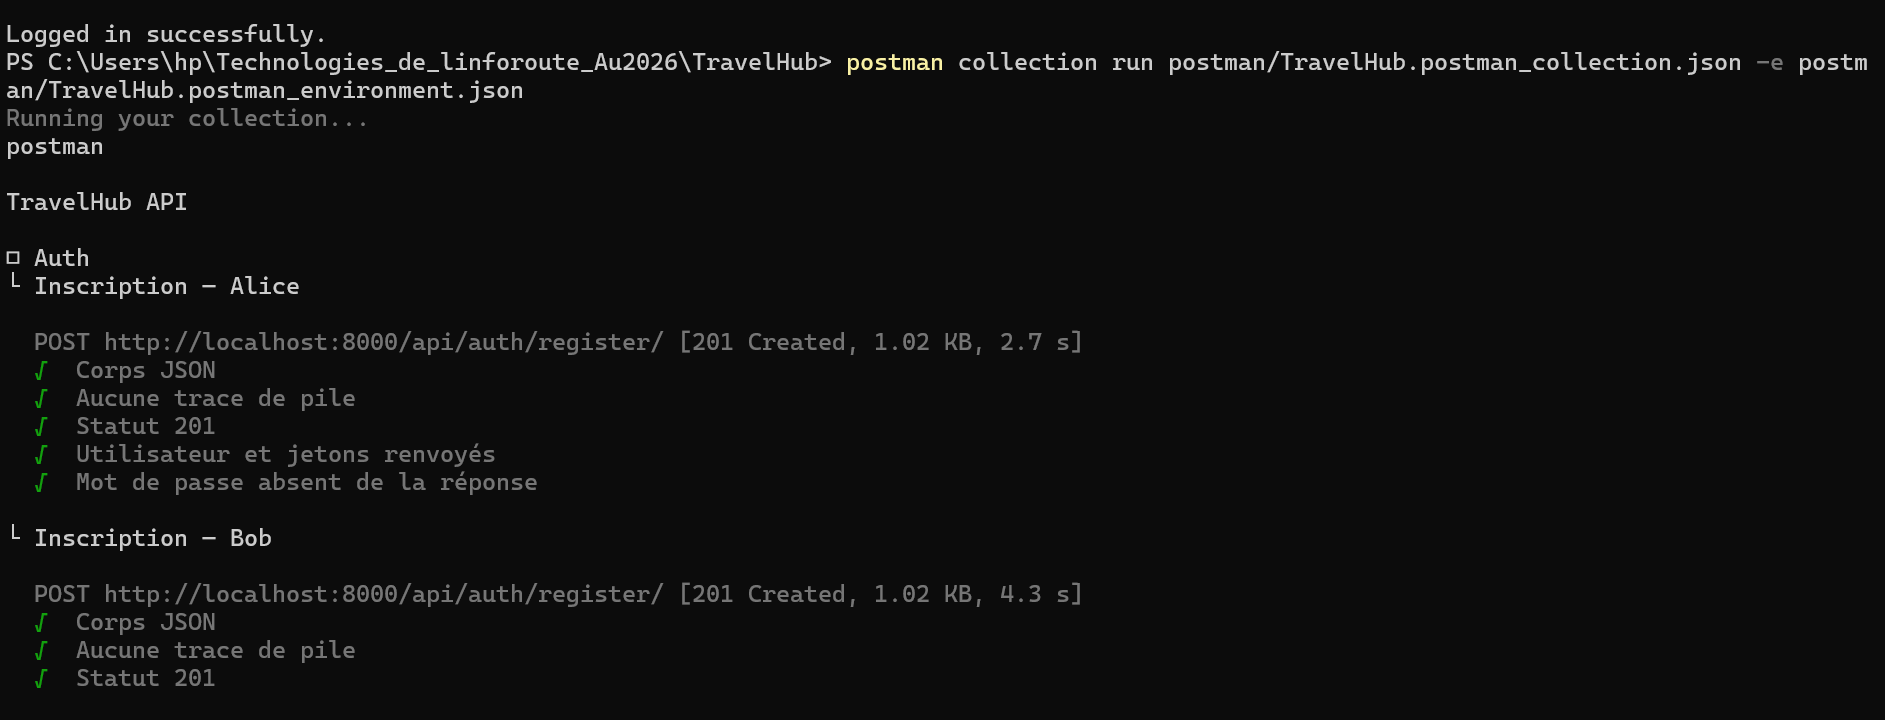
\includegraphics[width=\dimexpr\linewidth-2\fboxrule-2\fboxsep\relax]{figures/postman-runner.png}}%
  }{%
    \fbox{\parbox[c][3cm][c]{0.9\linewidth}{\centering\small
      Capture à insérer :\\[2pt] \texttt{figures/postman-runner.png}}}%
  }\\[6pt]
  \IfFileExists{figures/postman-runner1.png}{%
    \fbox{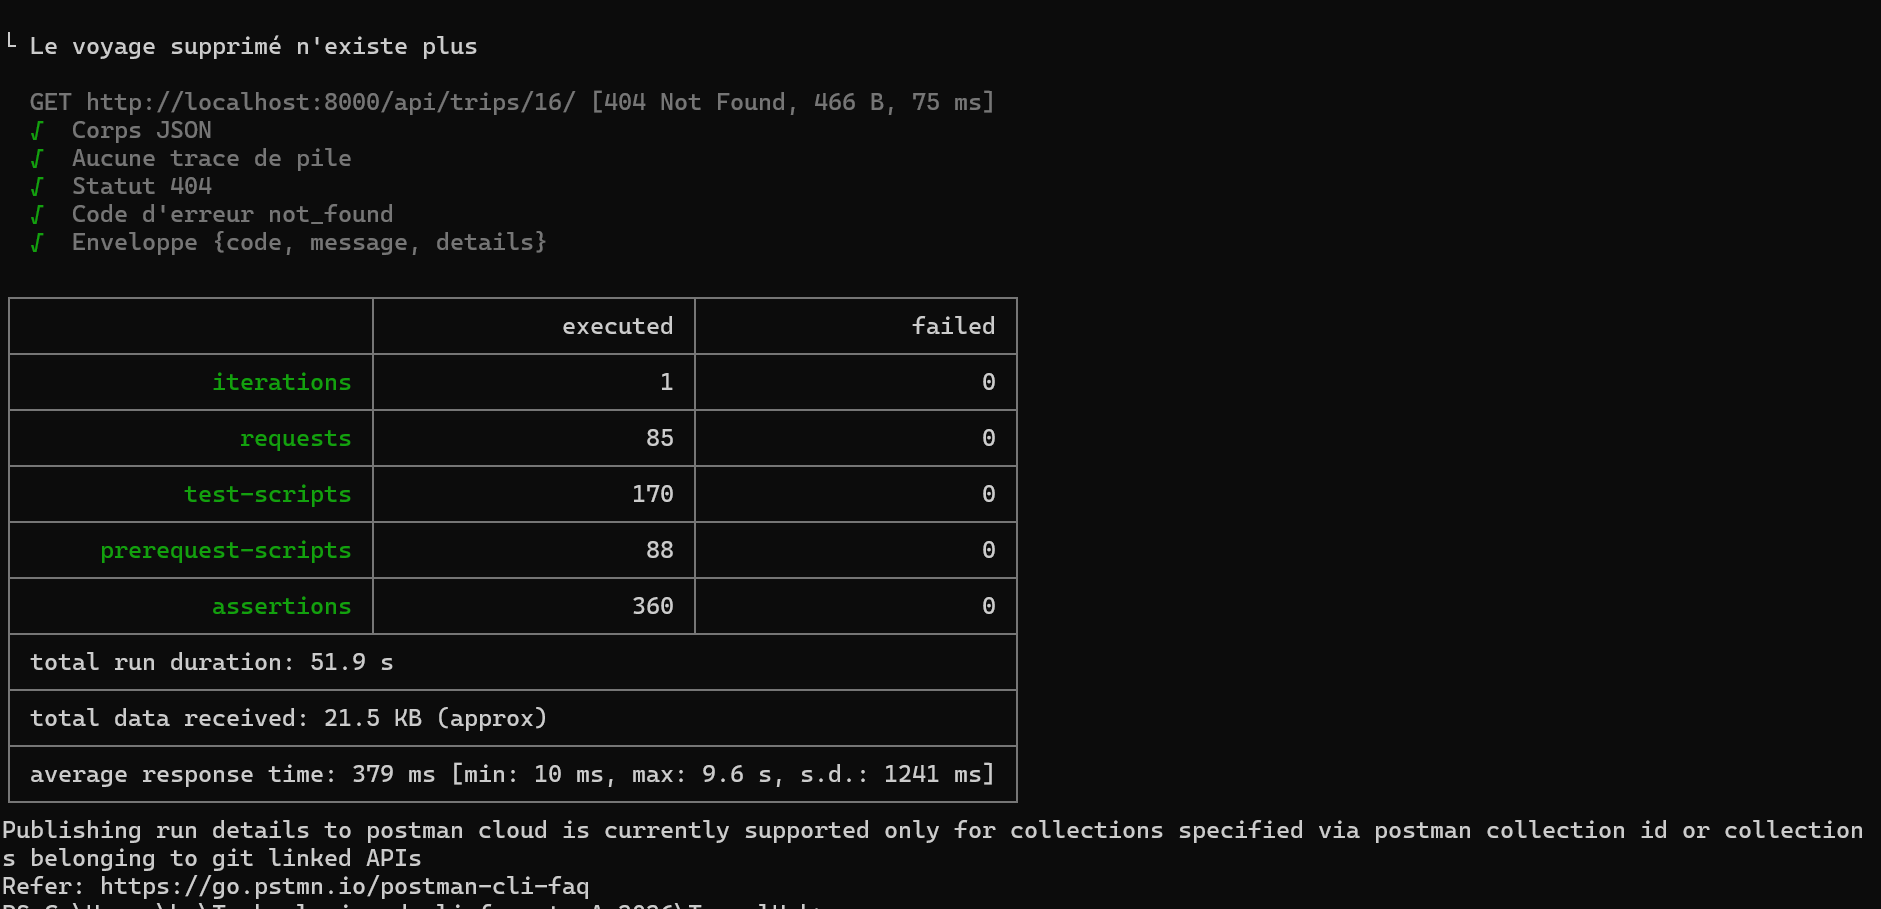
\includegraphics[width=\dimexpr\linewidth-2\fboxrule-2\fboxsep\relax]{figures/postman-runner1.png}}%
  }{%
    \fbox{\parbox[c][3cm][c]{0.9\linewidth}{\centering\small
      Capture à insérer :\\[2pt] \texttt{figures/postman-runner1.png}}}%
  }
  \caption{Exécution de la collection avec Postman CLI. En haut, le début de l'exécution avec les premières assertions. En bas, la dernière requête et le résumé (85 requêtes, 360 assertions, 0 échec).}
  \label{fig:postman}
\end{figure}

Les deux outils se complètent bien. Avec pytest, nous simulons les pannes qu'on ne peut pas provoquer quand on veut, comme un service externe en 500, un délai dépassé ou une panne au milieu d'une transaction. Postman, lui, vérifie le comportement de bout en bout, avec le vrai serveur et les vrais services externes.

\subsection{Qualité du code}

Ruff s'occupe de l'analyse statique (\code{ruff check}) et du formatage (\code{ruff format}). L'intégration continue lance ces deux vérifications avant les tests.

%========================================================================================
\section{Industrialisation}
\label{sec:industrialisation}
%========================================================================================

Cette partie va plus loin que l'énoncé. Nous l'avons faite seulement après avoir terminé tout ce qui était demandé.

\subsection{Docker}

Le \code{Dockerfile} construit l'image en deux étapes. La première part de \code{python:3.14-slim} et installe les dépendances dans un environnement virtuel. La deuxième copie cet environnement dans une image d'exécution qui n'a pas les outils de construction. L'image lance \code{collectstatic}, puis WhiteNoise sert les fichiers statiques. Gunicorn tourne avec un utilisateur sans privilèges, qui peut seulement écrire dans \code{/app/logs}. Une instruction \code{HEALTHCHECK} appelle \code{/health/} toutes les 30~secondes.

Le fichier \code{docker-compose.yml} regroupe trois services (tableau~\ref{tab:compose}).

\begin{table}[H]
  \centering
  \small
  \caption{Services Docker Compose.}
  \label{tab:compose}
  \begin{tabularx}{\linewidth}{@{}l X@{}}
    \toprule
    \textbf{Service} & \textbf{Rôle} \\
    \midrule
    \code{web} & Image du projet avec les paramètres de production. Applique les migrations puis lance Gunicorn, une fois que \code{db} est prêt \\
    \code{db} & \code{postgres:18} avec un volume persistant et un contrôle \code{pg_isready}. Le port n'est pas publié \\
    \code{pgadmin} & pgAdmin~4, accessible seulement depuis le poste local, avec le serveur TravelHub déjà déclaré \\
    \bottomrule
  \end{tabularx}
\end{table}

\subsection{Intégration continue}

Le flux GitHub Actions (\code{.github/workflows/ci.yml}) tourne à chaque \emph{push} sur \code{master} et à chaque \emph{pull request}. Il a deux tâches.

La première tâche s'appelle \og{}Lint et tests\fg{}. Elle démarre un service PostgreSQL 18, puis Ruff vérifie le code et son formatage. Pytest est lancé ensuite avec le seuil de couverture de 80\,\%. Le résumé de couverture s'affiche sur la page de l'exécution et les rapports sont publiés comme artefacts.

La deuxième tâche construit l'image Docker avec un cache et la démarre avec \code{docker compose up --wait}. Elle vérifie ensuite que \code{/health/}, \code{/api/docs/} et \code{/api/schema/} répondent.

Dependabot propose aussi chaque semaine les mises à jour des dépendances pip et des actions GitHub. La figure~\ref{fig:ci} montre l'historique des exécutions. Elles ont toutes réussi, y compris celles lancées par les pull requests de Dependabot.

\capture{ci-github.png}{Historique du flux CI sur GitHub Actions. Les six exécutions ont réussi.}{fig:ci}

\subsection{Journaux et contrôle de santé}

Chaque événement donne une ligne JSON, écrite sur la console et dans un fichier rotatif (10~Mo, 5~archives). L'intergiciel \code{RequestIdMiddleware} donne un identifiant à chaque requête. On le retrouve dans toutes les lignes de journal de la requête et dans l'en-tête \code{X-Request-ID} de la réponse. Si un utilisateur signale une erreur, une seule recherche suffit pour la retrouver.

\begin{lstlisting}[language=json,caption={Ligne de journal d'une requête.},label={lst:log}]
{"timestamp": "2026-10-23T22:01:39.510+00:00", "level": "INFO", "logger": "travelhub.request",
 "message": "GET /api/trips/ 200", "request_id": "292f04c8d5e541e69c07c7565e0e65f0",
 "method": "GET", "path": "/api/trips/", "status": 200, "duration_ms": 401.1, "user_id": 5}
\end{lstlisting}

Le point d'accès \code{/health/} vérifie la base avec \code{SELECT 1} et le cache avec une écriture suivie d'une lecture. Il répond 200 si tout va bien et 503 sinon. La cause de l'échec n'est pas donnée au client, mais elle est écrite dans les journaux.

\subsection{Sauvegarde et restauration}

Les scripts \code{scripts/backup.ps1} et \code{scripts/restore.ps1} utilisent \code{pg_dump} et \code{pg_restore}. Ils marchent pour la base locale et pour celle du conteneur. Chaque archive est relue avant d'être gardée, et on ne garde que les sept plus récentes. La restauration se fait dans une seule transaction, donc une archive corrompue ne touche pas la base. Une base qui n'est pas vide n'est écrasée qu'avec l'option \code{-Force}. Pour vérifier une sauvegarde, nous la restaurons dans une base neuve et nous contrôlons le schéma avec \code{migrate --check}.

%========================================================================================
\section{Conclusion}
\label{sec:conclusion}
%========================================================================================

\subsection{Bilan}

Le back-end de TravelHub répond à tout l'énoncé. Le modèle relationnel a des relations 1-N et une relation N-N avec ses propres attributs, et PostgreSQL vérifie les règles importantes. Les mêmes fonctions sont disponibles dans une API REST documentée avec OpenAPI et dans une API GraphQL. Les deux partagent la logique métier, les permissions et la validation. Les deux services externes sont appelés avec un délai, un nouvel essai, un cache et une dégradation partielle. Pour la sécurité, nous avons suivi l'OWASP API Security Top 10, et 724 tests automatisés couvrent 98\,\% du code.

Quelques choix nous ont beaucoup aidés. Comme toutes les requêtes partent de \code{visible_to()}, le contrôle d'accès au niveau objet est réglé une seule fois, et pas vue par vue. Valider à la fois dans l'application et dans la base nous donne des erreurs claires, tout en gardant les données cohérentes quand deux requêtes arrivent en même temps. Enfin, grâce aux services métier partagés, ajouter l'API GraphQL n'a demandé qu'une nouvelle couche de présentation.

\subsection{Limites}

Notre travail a quand même des limites. En production, nous n'avons pas configuré de moteur de cache. Django utilise donc un cache en mémoire propre à chaque processus. Les réponses externes et les compteurs de limites de requêtes ne sont pas partagés entre les processus Gunicorn. Avec deux processus, la limite réelle est donc deux fois plus haute.

Les prévisions météo ne vont pas au-delà de 16 jours, et Countries donne les noms de pays seulement en anglais. Les risques résiduels de la section~\ref{sec:securite} sont toujours là (on peut deviner des courriels, la largeur des requêtes GraphQL n'est pas limitée, la documentation OpenAPI est publique). Enfin, la pagination GraphQL par décalage devient lente sur de très grandes listes. Une pagination par curseur serait plus solide.

\subsection{Pistes pour le TP2}

Le front-end pourra utiliser directement ce que nous avons fait. GraphQL servira pour les écrans les plus chargés, comme la page d'un voyage avec la météo et le pays, en une seule requête. Il faudra seulement ajouter son origine à \code{CORS_ALLOWED_ORIGINS}. Avec les codes d'erreur stables et le champ \code{details}, on pourra afficher chaque message à côté du bon champ de formulaire. L'en-tête \code{X-Request-ID} permettra aussi de retrouver dans les journaux une erreur vue par l'utilisateur. Côté serveur, un cache partagé comme Redis réglerait la principale limite que nous avons relevée.


\newpage
\bibliography{report_v1.0}


\end{document}
